
\begin{figure*}[t]
        \centering
        \begin{minipage}{0.3\textwidth}
                \centering
                \includegraphics[width=\textwidth]{graphs/cdf-layer-repull-ratio-by-same-client.pdf}
                \caption{CDF of \texttt{GET} layer request count}
                \label{fig:layer-repull-cdf}
        \end{minipage}%
	\hfill
        \begin{minipage}{0.265\textwidth}
                \centering
                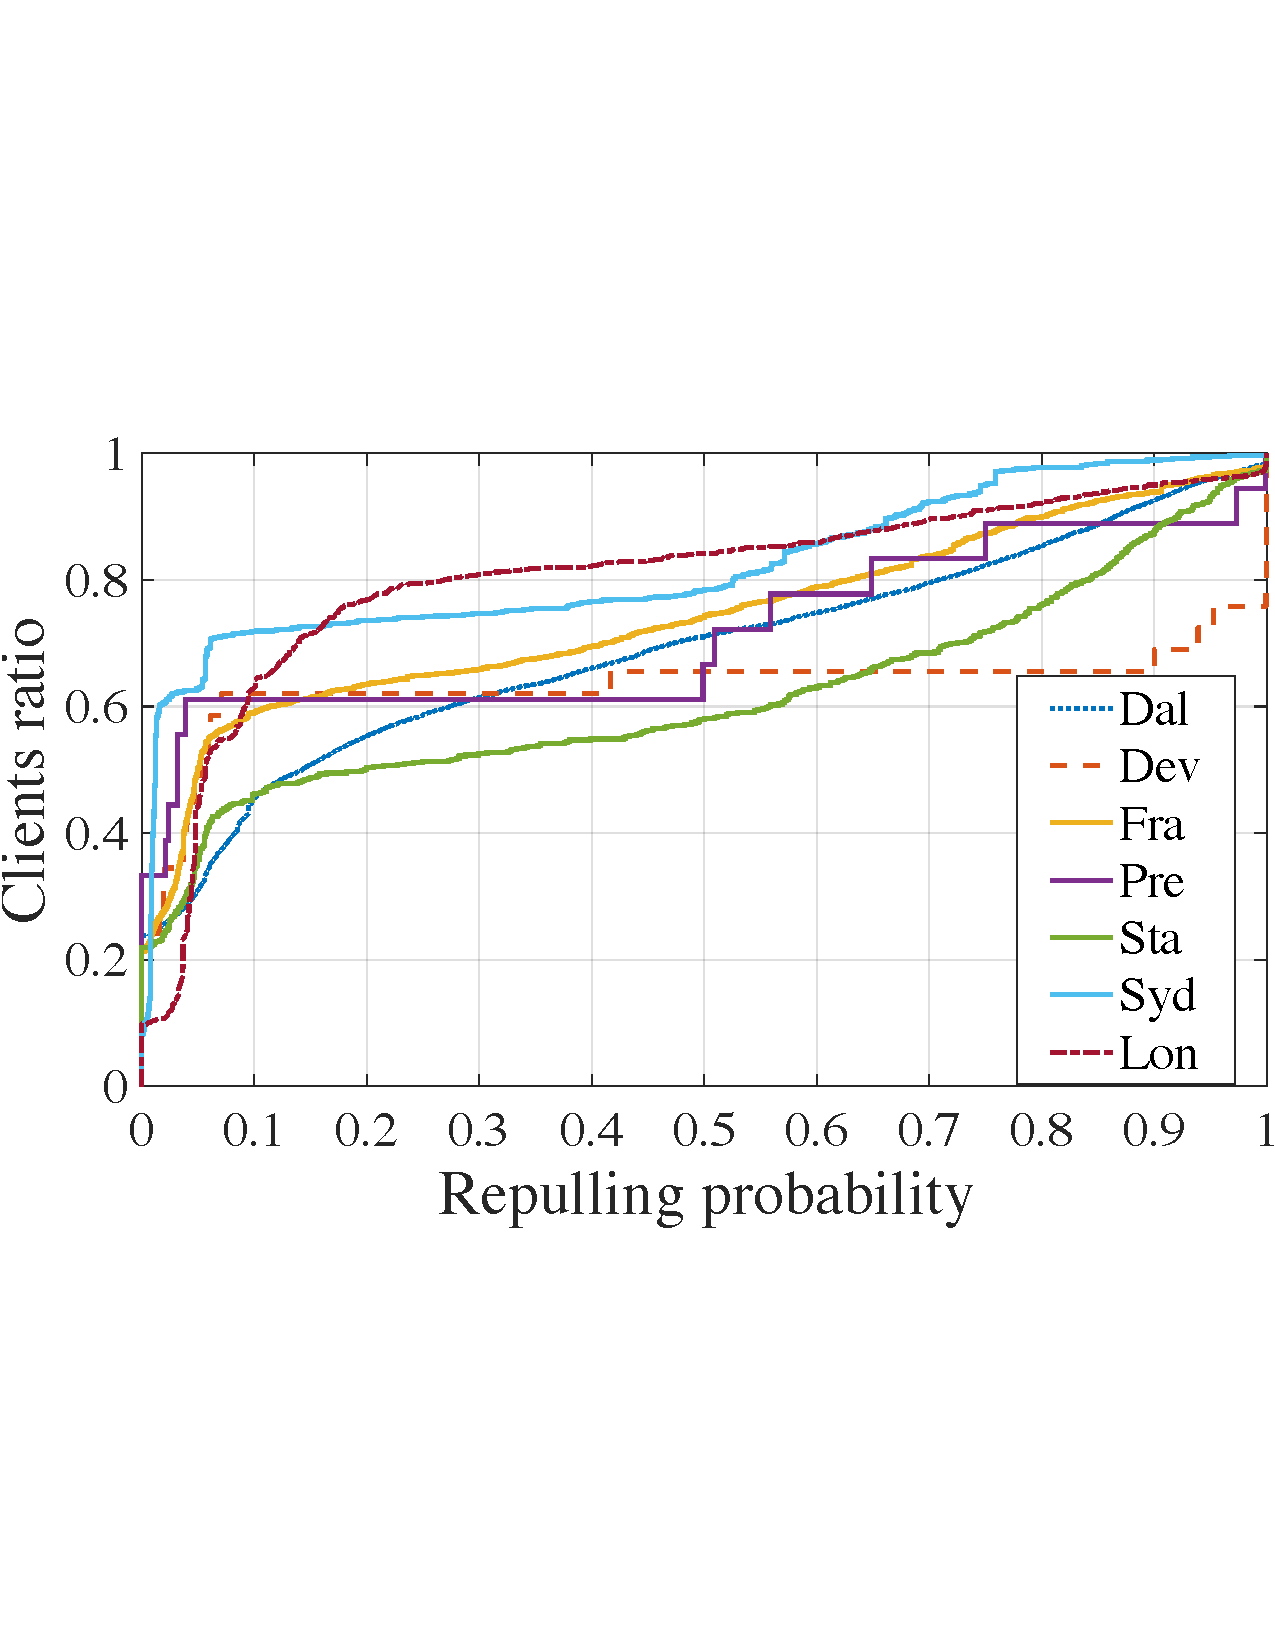
\includegraphics[width=\textwidth]{graphs/cdf-client-repull-layer-request-ratio.pdf}
                \caption{CDF of Client repulling probability}% of LRU cache and preconstruct cache.}
                \label{fig:client-repull-cdf}
        \end{minipage}%
	\hfill
        \begin{minipage}{0.25\textwidth}
        \centering
        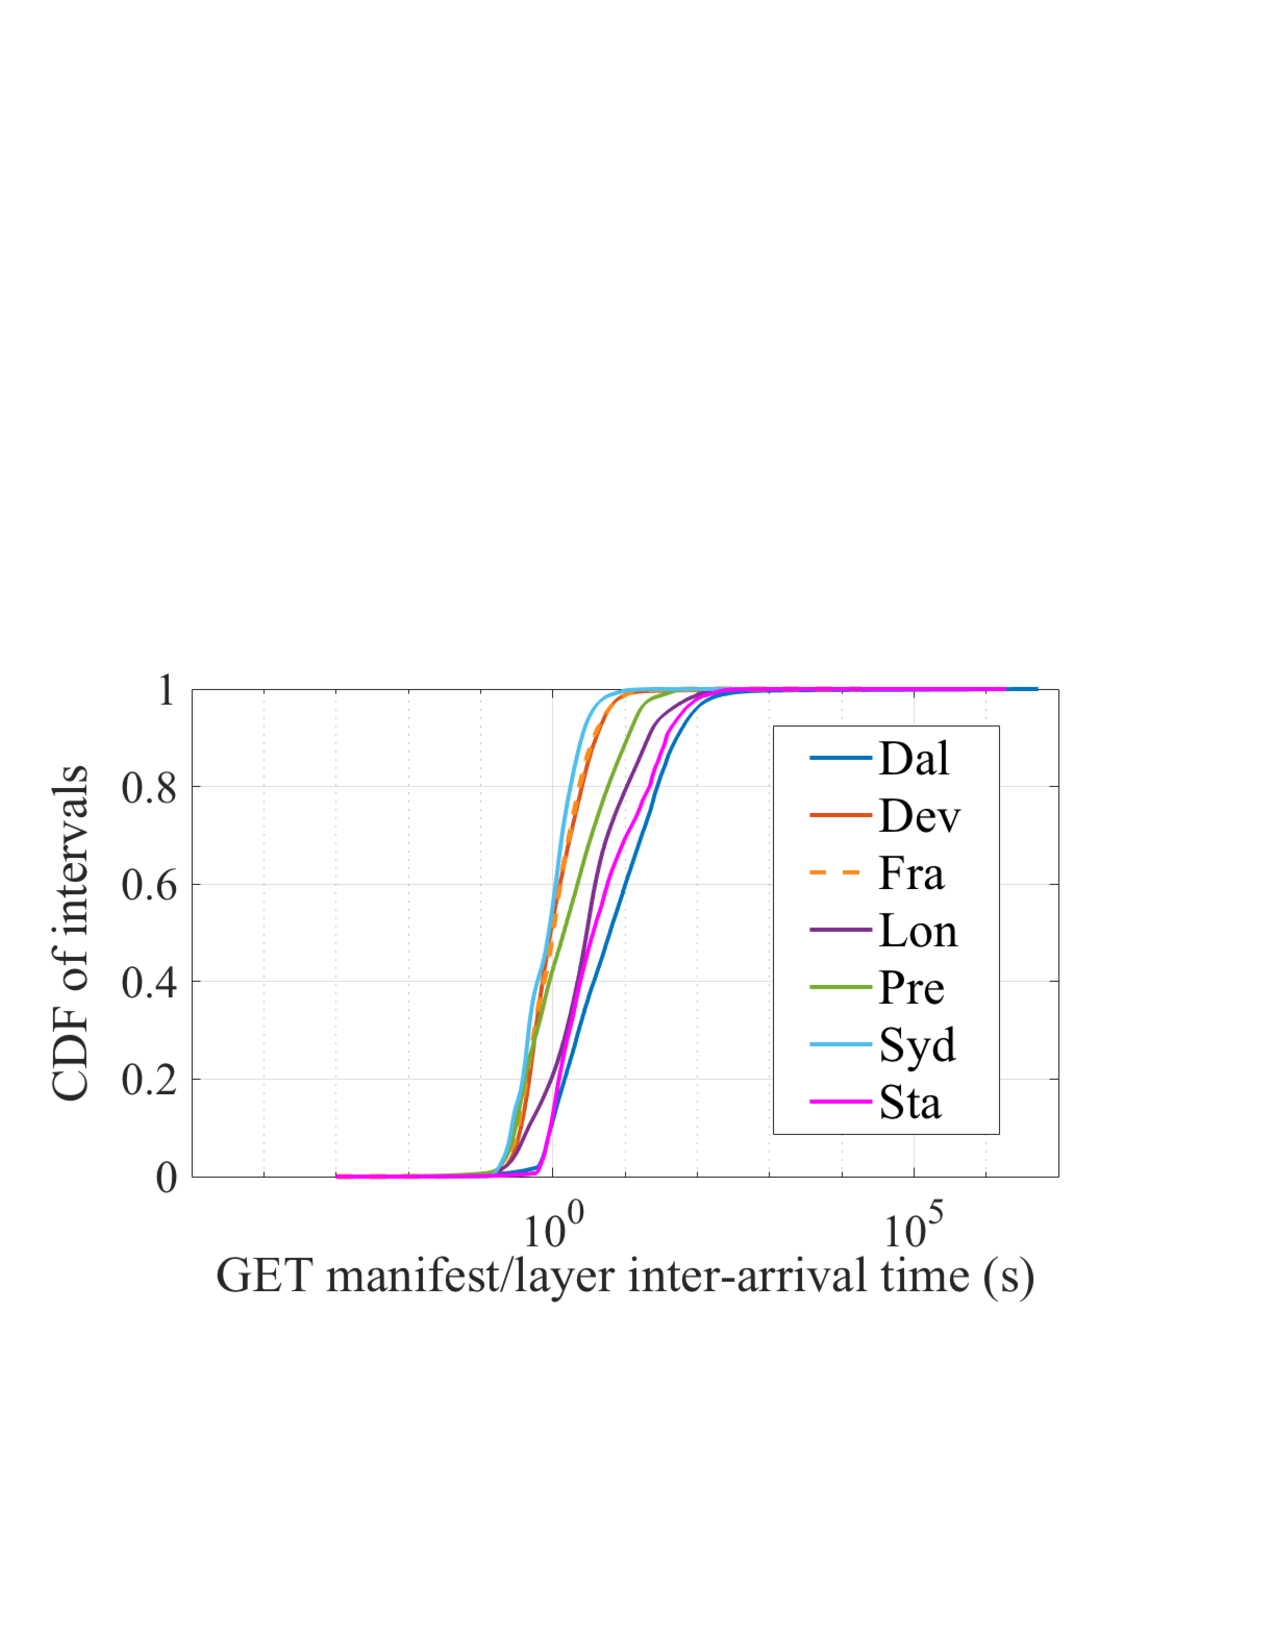
\includegraphics[width=\textwidth]{graphs/GML-intervals.pdf}
        \caption{CDF of \texttt{GET} manifest/layer IAT}
        \label{fig:intervals}
        \end{minipage}
\end{figure*}



\section{Motivation and Challenges}
\label{sec:dataset-analysis}

In this section we first explore why file-level deduplication in Docker
registries can effectively reduce storage
utilization~(\S\ref{sec:inter-layer-deduplication}).
%
We then discuss the feasibility of predicting and exploiting registry access
patterns for proactive layer restoration~(\S\ref{sec:predictable-user-access}).
%before they are requested~(\S\ref{sec:layer-preconstruction}) to reduce the
%deduplication overhead for layer retrievals.

\subsection{Inter-layer Data Redundancy}
\label{sec:inter-layer-deduplication}

Layers inside different container images exhibit a large amount of redundancy
in terms of duplicate files.
%
Although Docker
%uses copy-on-write file systems to minimize redundant data inside each image and
supports the sharing of layers among different images to remove some redundant data in the
Docker registry,
%a large amount of duplicated files are observed among layers within different images.
this is not sufficient to effectively eliminate duplicates.
%
According to the deduplication analysis of the Docker Hub
dataset~\cite{dedupanalysis}, only 3.2\% of files are unique, resulting in
a deduplication ratio of 2$\times$ in terms of
capacity\footnote{The deduplication ratio is 2$\times$ despite the 97\% of redundant data
because many of the unique files are large in size.}.
%
We believe that the deduplication ratio is much higher when
private registries are taken into account.
%
The duplicate files
%shared among different layers associated with different images
are executables, object codes, libraries, and
source codes, and are likely imported by different image developers using the
package installers or version control systems such as \texttt{apt},
\texttt{pip} or \texttt{git} to install similar dependencies.
% or source codes.  
%
This file-level redundancy cannot be eliminated by the current layer-level content addressable
storage system design.

As containerization frameworks like Docker keep gaining more
popularity, more applications are encapsulated into images and pushed into
registries.
%, and stored on Cloud.
%
$R$-way replication for reliability additionally fuels the high storage demands
of Docker registries.
%the amount of layers data grows exponentially and will explode in future.
%
Hence, satisfying the demand by adding more disks and scaling out storage systems
quickly becomes expensive.
%due to the rapid growth of images.
%This large volume data management challenge can not be solved by just adding
%more disks and goes beyond just hardware upgrade or even datacenter expansion.
%such as missive and slow data migration during scale-out or scale-up.
 
File-level deduplication can address this challenge reducing the need of storage expansion.
%
A deduplication solution needs to first decompress
the compressed layer tarballs and then remove the duplicate files across
different layers.
%
%This way, the layer dataset stored in the registry can be largely reduced for more
%effective storage utilization.
%data management.
%
However, retrieving a layer from a registry with file-level
deduplication support requires restoring the layer,
which involves fetching the files, archiving and compressing them\footnote{Notice
that given the large variety of Docker clients the registry-side enhancements
should not involve changes on the client-side.}.
%
These extra operations incur a considerable overhead for
\texttt{GET} layer requests, which already constitute a significant portion of
the container startup time~\cite{slacker}.
%
In this paper, we explore if it is possible to deduplicate layers and save storage space
without sacrificing the \texttt{GET} layer performance.
%   
%Consider that deduplication incurs a performance overhead and the current
%Docker registry already stores layers in compressed format to save space and
%network transfer overhead. We first analyze the space efficiency of a registry
%that performs decompression and file-level deduplication and compare it to a
%registry that naively stores compressed layers.

%In Figure~\ref{fig:cacheefficiency}, the x-axis values correspond to the sizes
%of $5$ samples of registry data of varying sizes with traditional layer
%compression. For a traditional registry, the compressed layer tarballs will be
%kept as is.  While a registry with file-level deduplication will store
%\emph{deduplicated} layers (i.e., unique files).  The y-axis shows how much
%space a registry with file-level deduplication can save over compressed layer
%tarballs.  For the first two samples of the dataset, with size less than
%$20$~GB, there is no benefit to \emph{deduplicate} layers because the
%deduplication ratio is very low.  However, when the dataset size is $200$~GB
%and over, we can save over $40\%$ more space increasing almost linearly with
%the size of the layer dataset.  This verifies the benefit of deduplicating
%layers as the registry size increases.  Before describing Sift, we must
%understand the storage pressure and trends in the access patterns of the
%Docker registries at the layer and repository level.

\subsection{Predictable User Access Patterns}
\label{sec:predictable-user-access}


%%\begin{figure*}[t]
%		\begin{minipage}{0.32\linewidth}
%			\centering
%			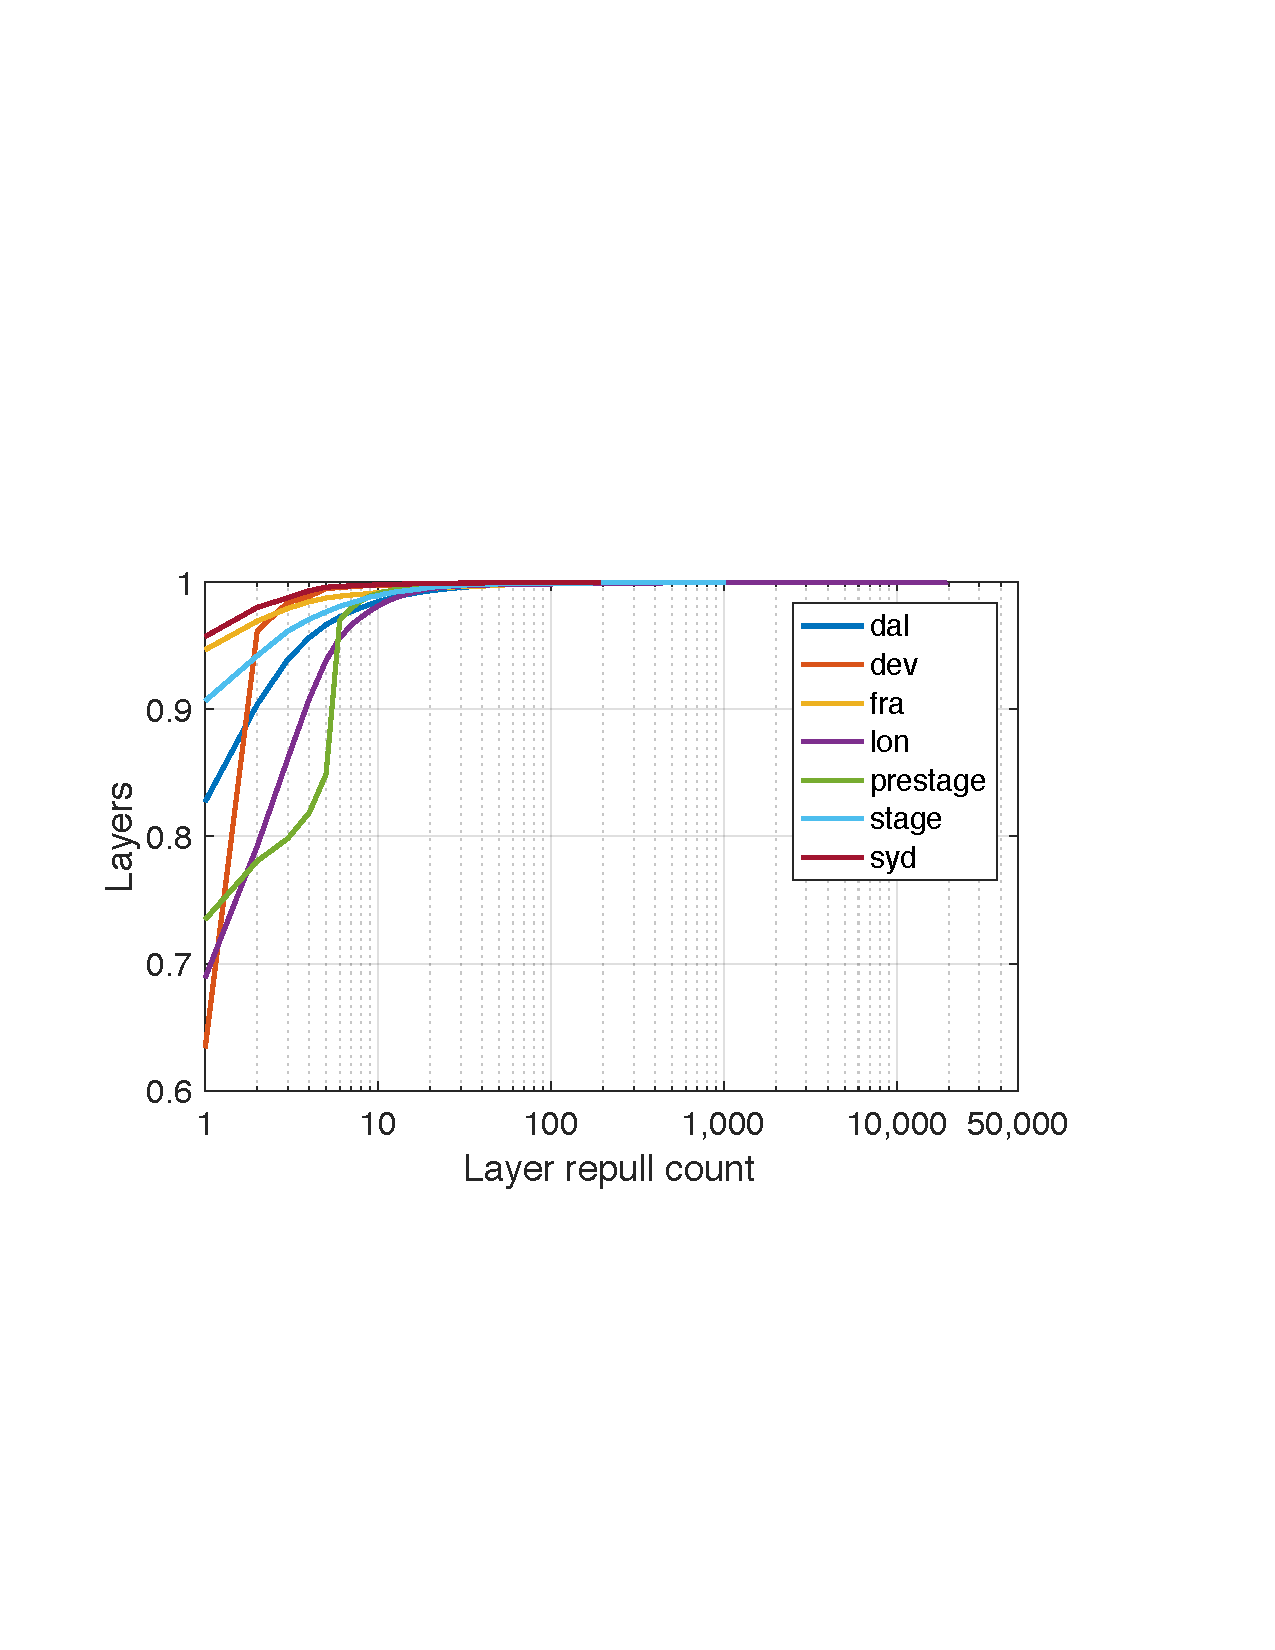
\includegraphics[width=1\textwidth]{graphs/cdf-layer-repull-by-same-client.pdf}
%			%\caption{CDF of layer repull count.}
%		%	\vspace{-3pt}
%			\label{fig:layer-repull-cdf}
%		\end{minipage}
%			\begin{minipage}{0.32\linewidth}
%				\centering
%				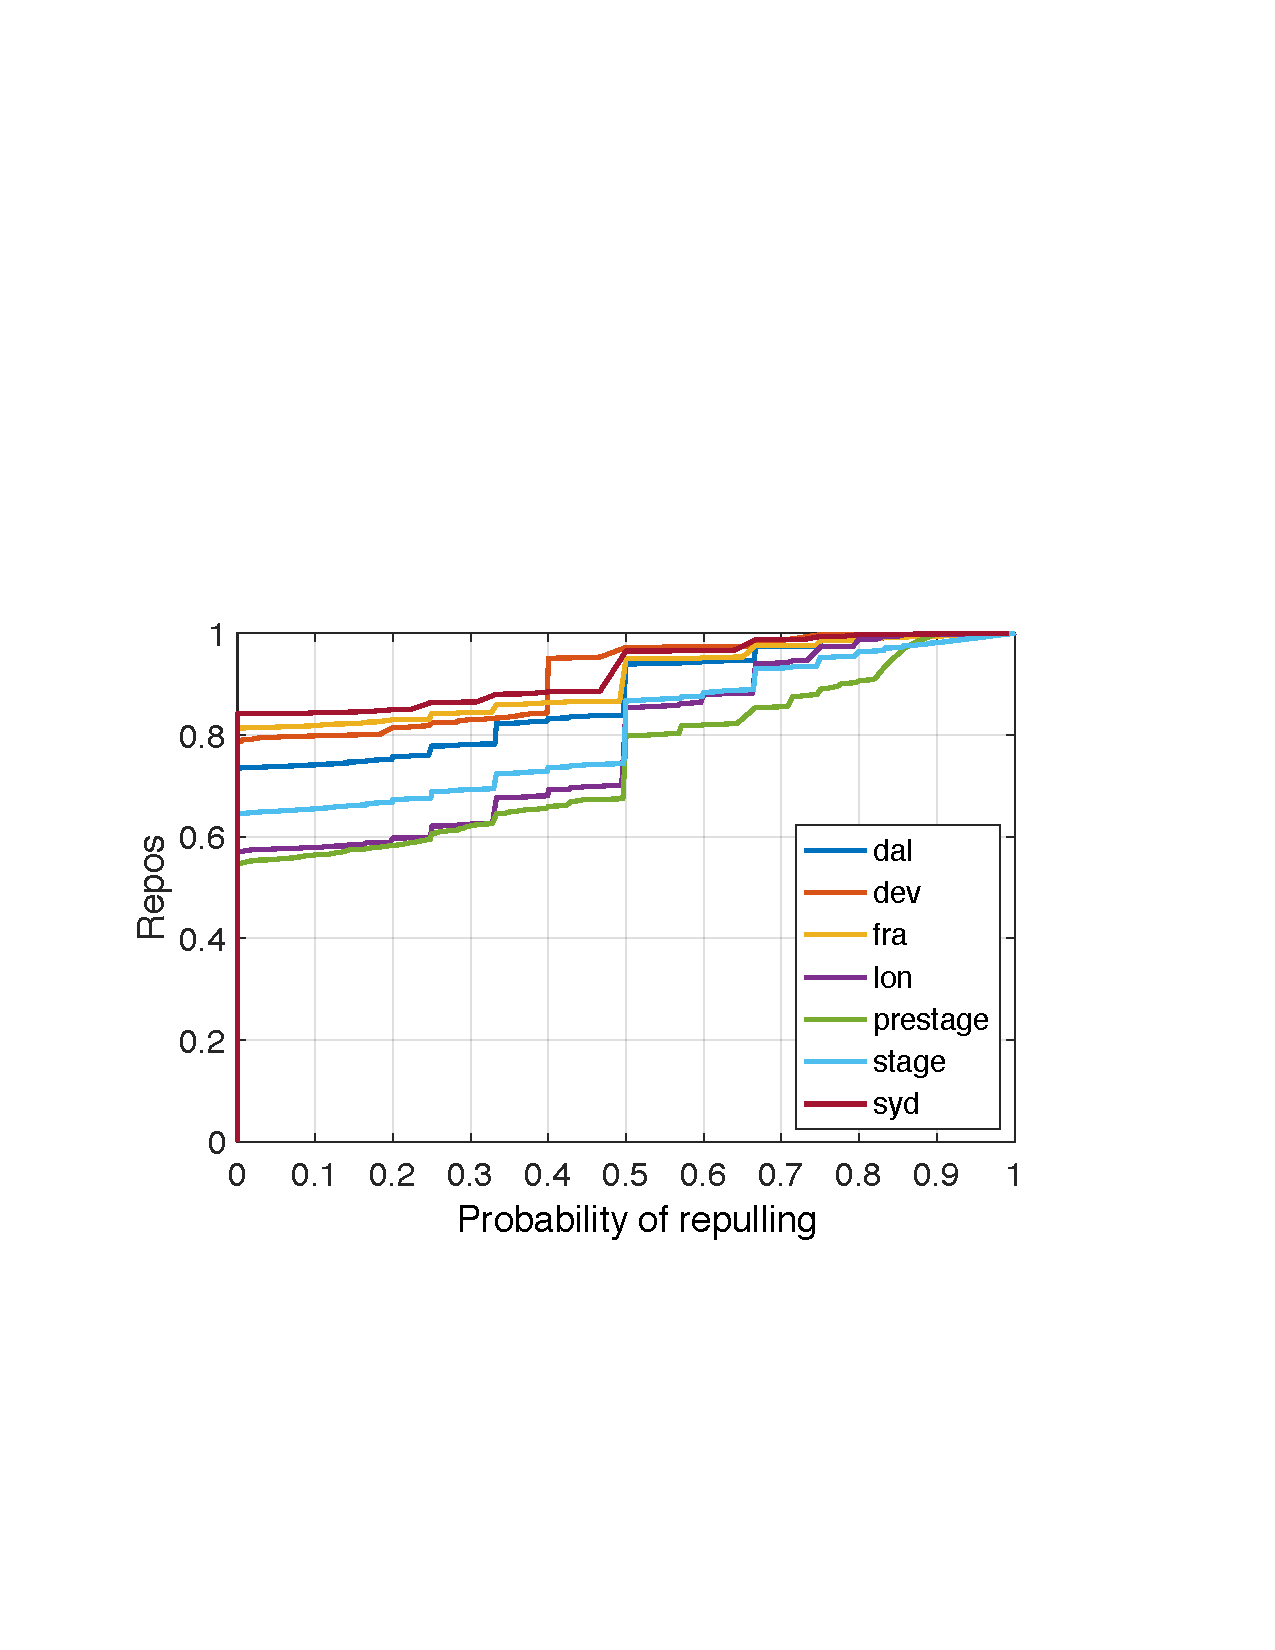
\includegraphics[width=1\textwidth]{graphs/cdf-repo-repull-ratio-by-same-client.pdf}
%				%\caption{PDF of repository repulling probability.}
%				%	\vspace{-3pt}
%				\label{fig:repo-repull-cdf}
%			\end{minipage}
%		\begin{minipage}{0.32\linewidth}
%			\centering
%			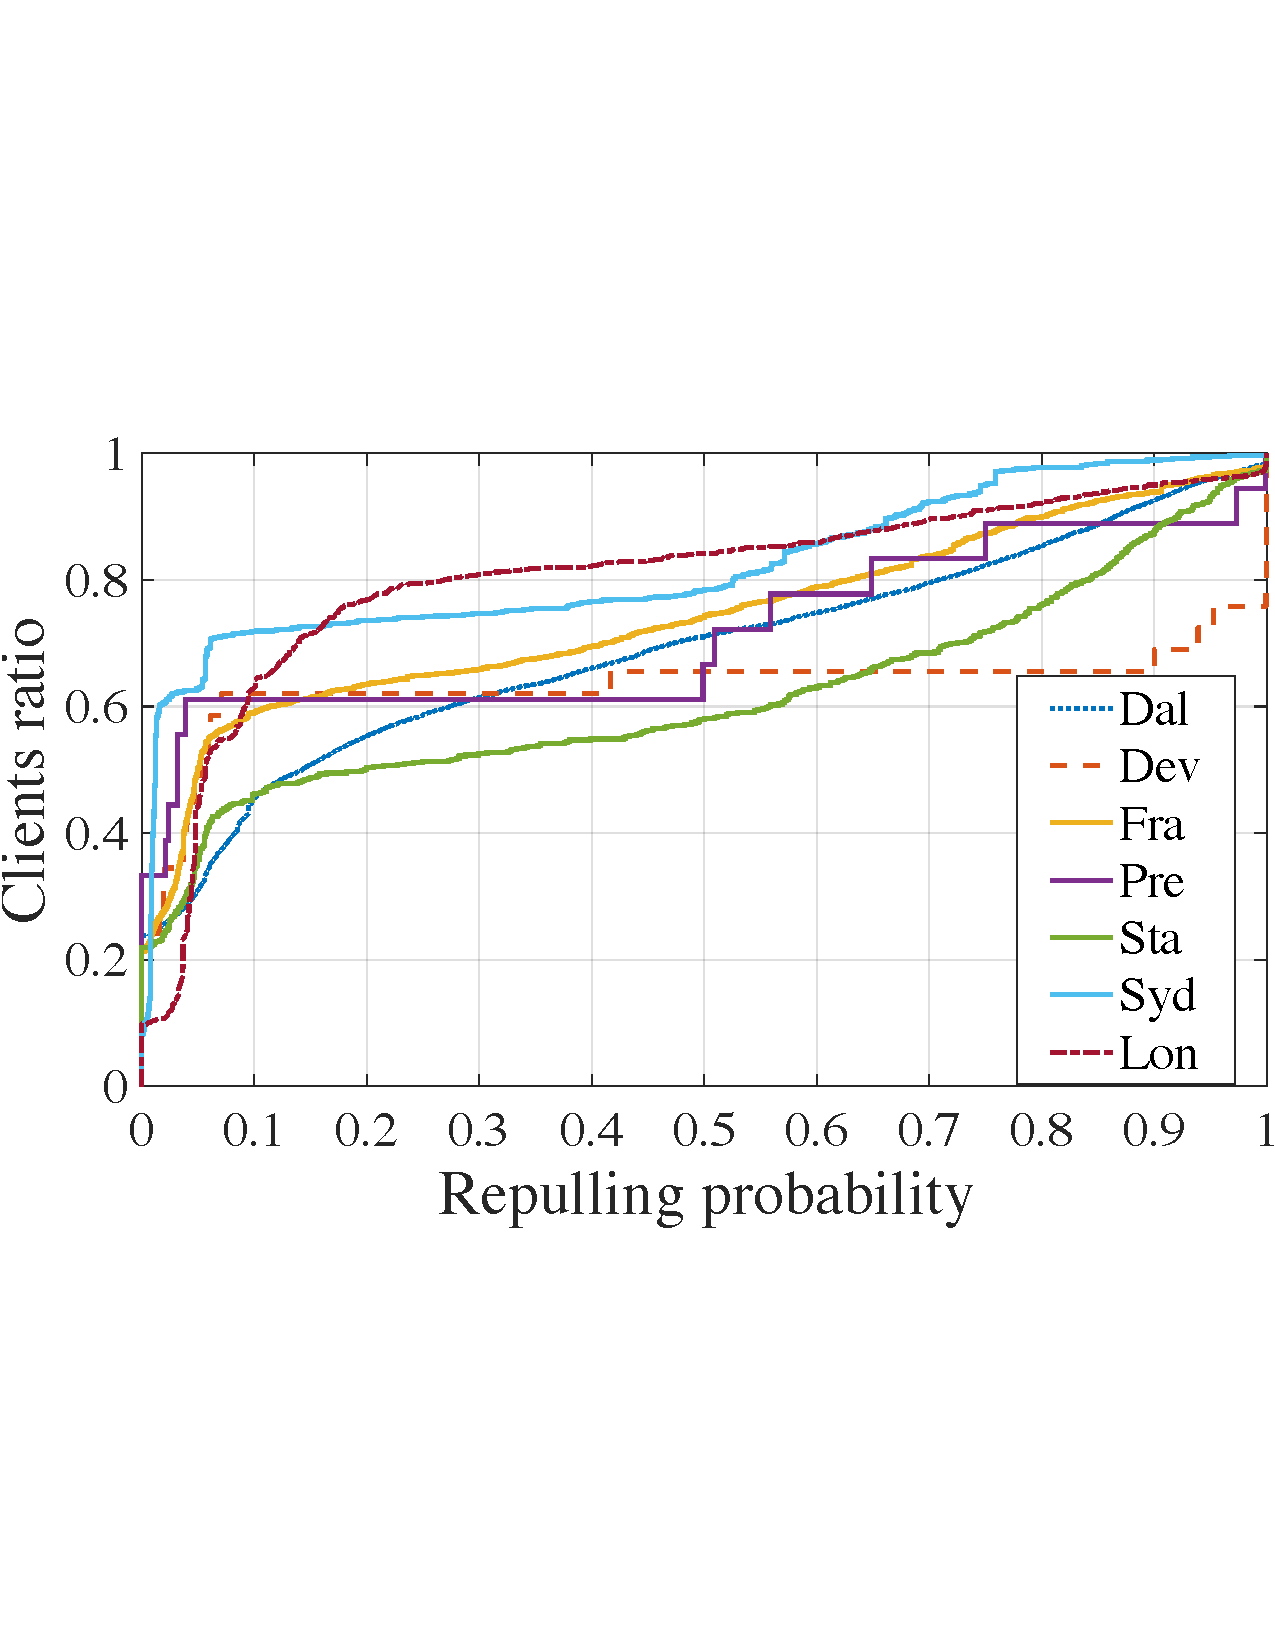
\includegraphics[width=1\textwidth]{graphs/cdf-client-repull-layer-request-ratio.pdf}
%			%
%			%	\vspace{-3pt}
%			\label{fig:client-repull-cdf}
%		\end{minipage}
%	\caption{PDF of client repull count, repository repulling probability, and client repulling probability..}
%\end{figure*}

%\begin{figure}[!t]
%	\centering
%	\subfigure[\texttt{GET} layer request count]{
%		\includegraphics[width=0.22\textwidth]{graphs/cdf-layer-repull-ratio-by-same-client.pdf}
%		\label{fig:layer-repull-cdf}
%	}
%%	\subfigure[Repository repulling probability]{
%%		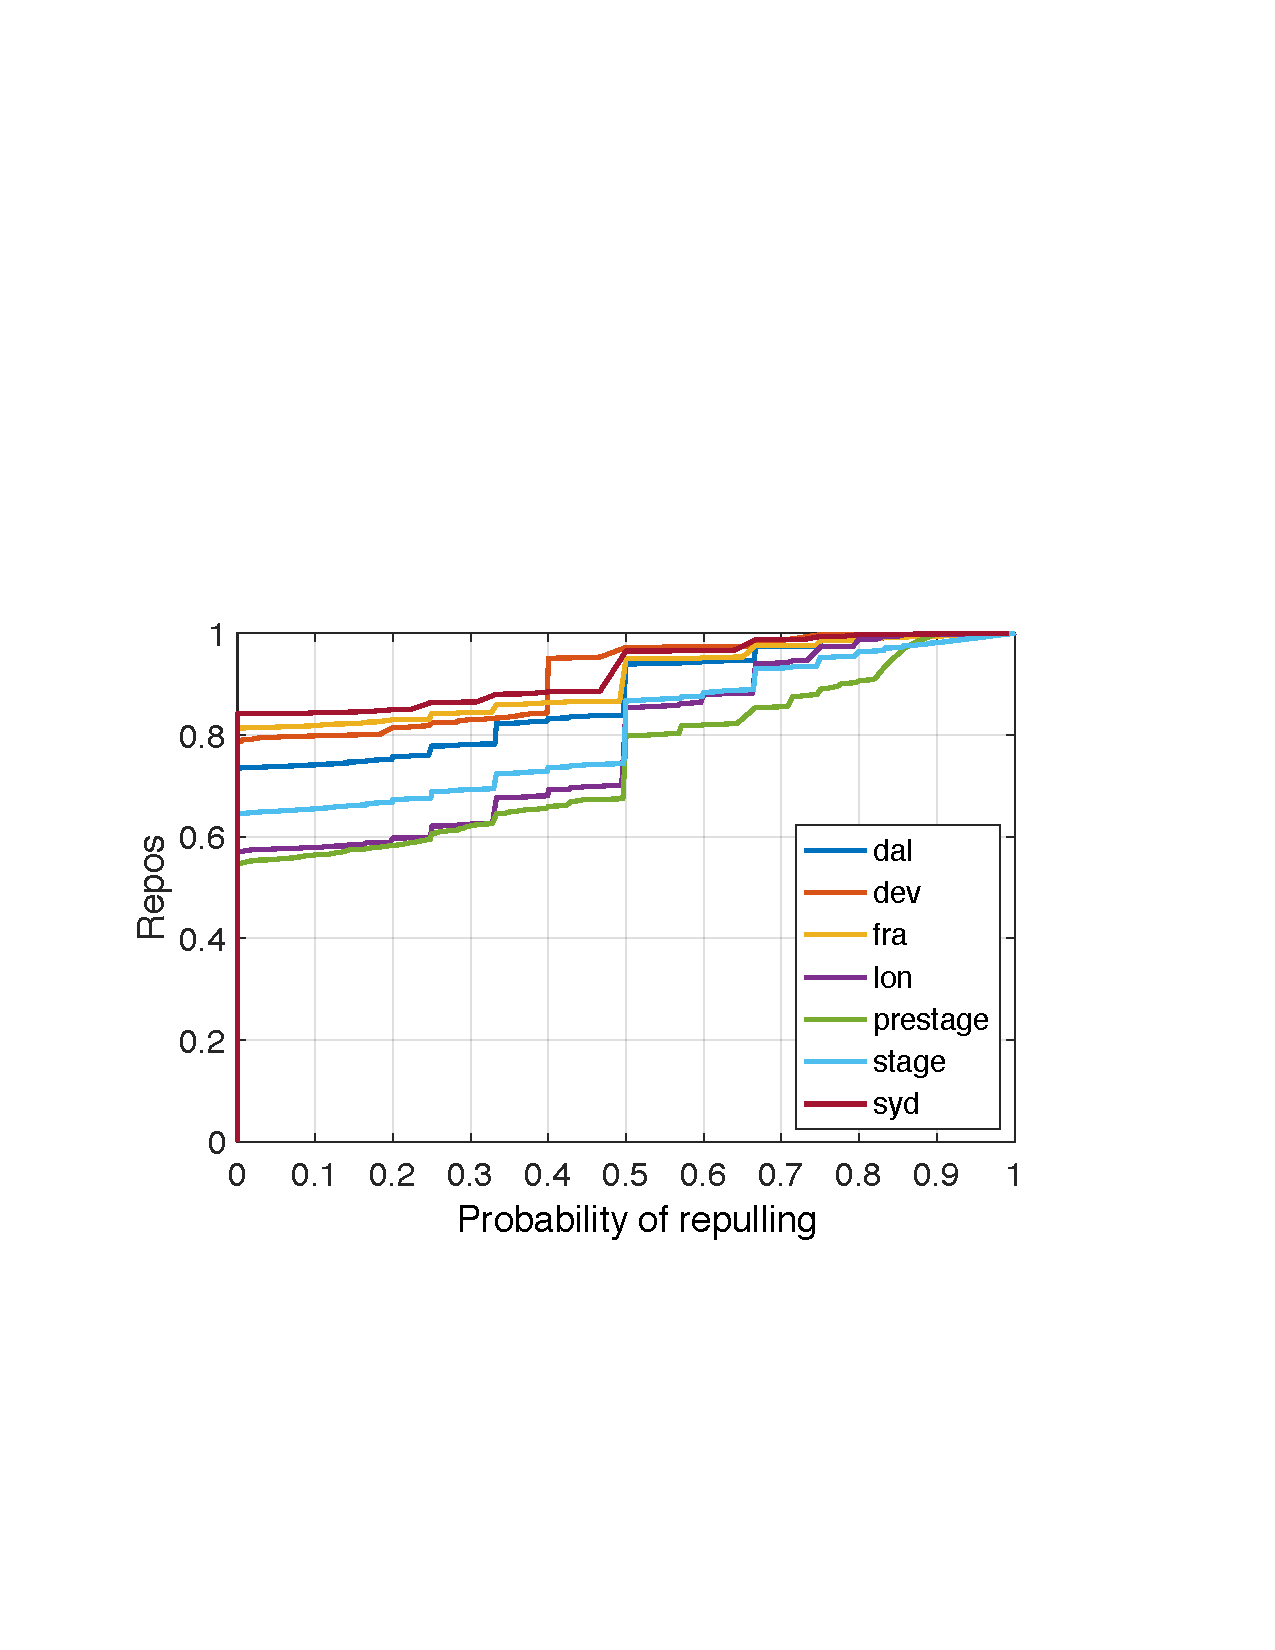
\includegraphics[width=0.2\linewidth]{graphs/cdf-repo-repull-ratio-by-same-client.pdf}
%%		\label{fig:repo-repull-cdf}
%%	}
%	\subfigure[Client repulling probability]{
%	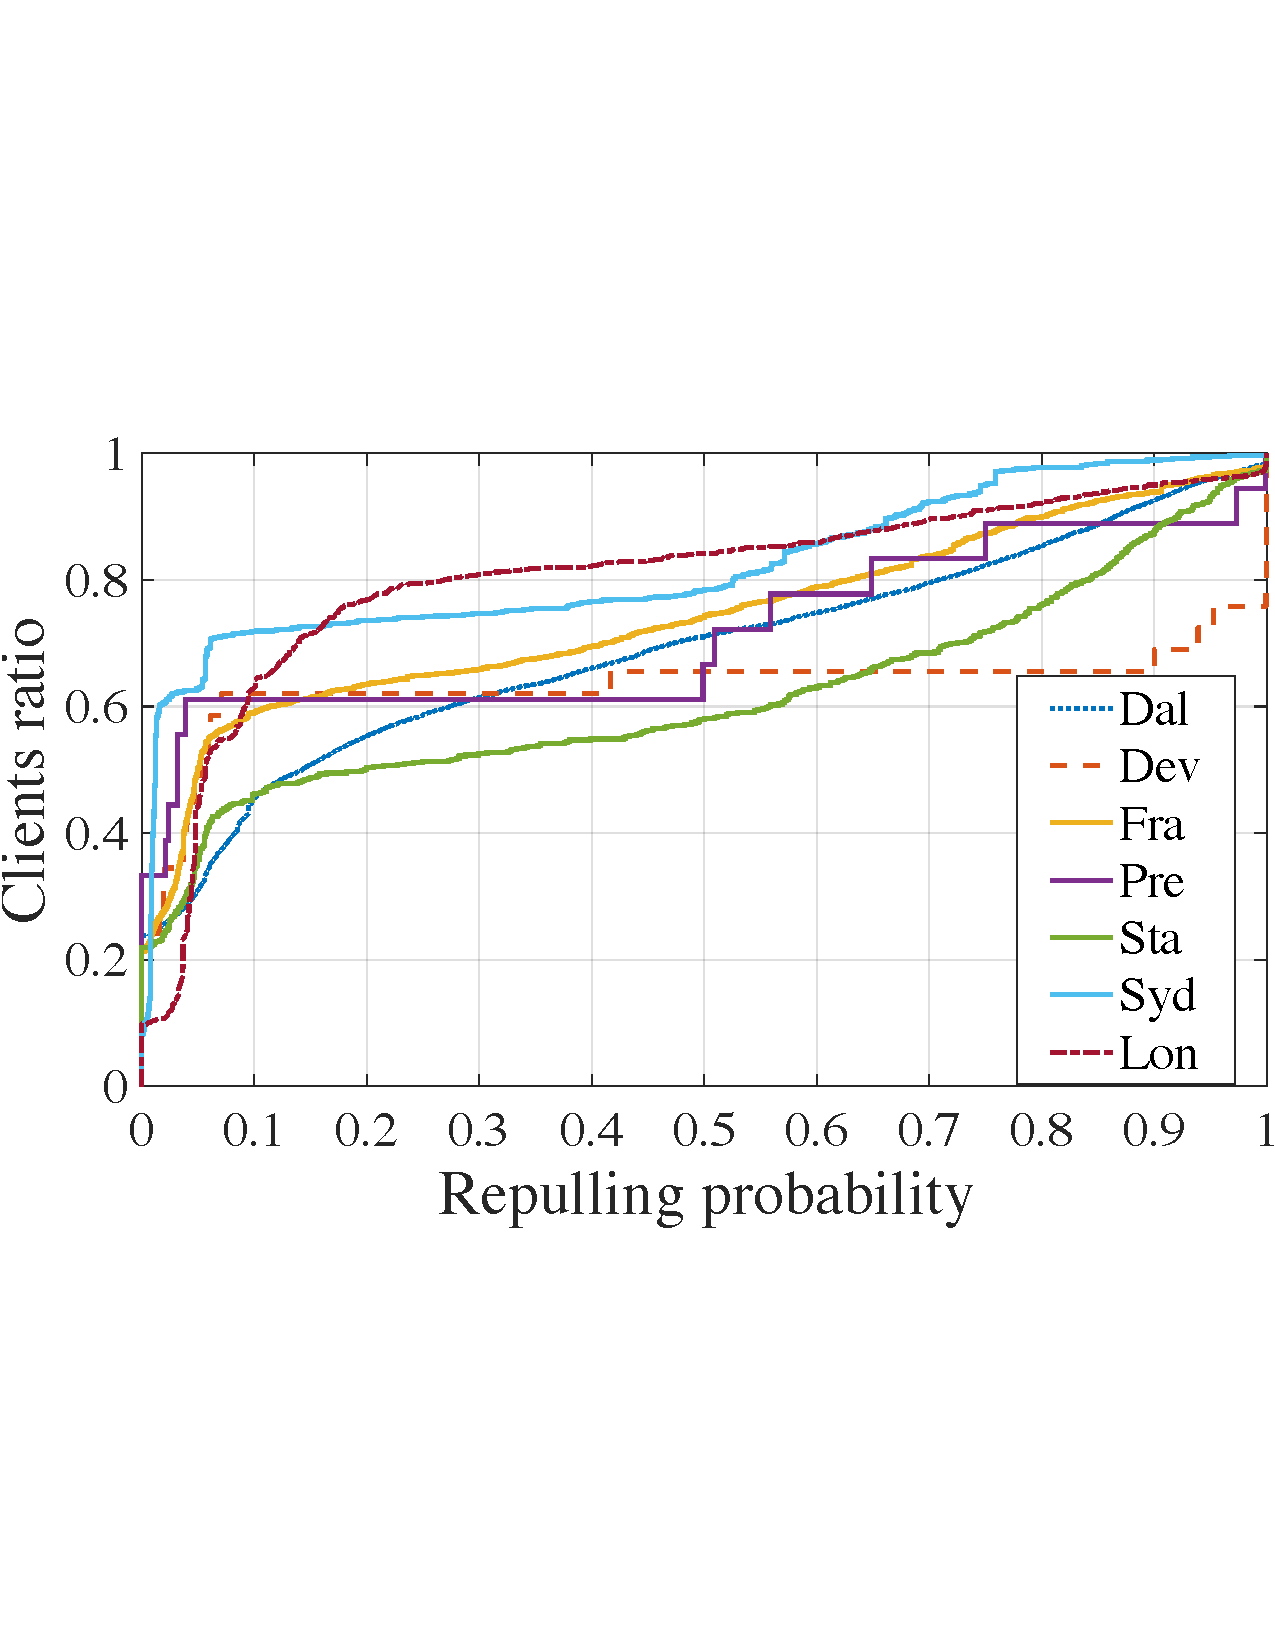
\includegraphics[width=0.2\textwidth]{graphs/cdf-client-repull-layer-request-ratio.pdf}
%   \label{fig:client-repull-cdf}
%}
%	\caption{CDF of \texttt{GET} layer request count and client repulling probability.}
%	\label{fig-repull}
%\end{figure}
%






\begin{figure*}[t]
        \centering
        \begin{minipage}{0.3\textwidth}
                \centering
                \includegraphics[width=0.9\textwidth]{{graphs/cdf-layer-repull-ratio-by-same-client.pdf}
                \caption{CDF of \texttt{GET} layer request count}
                \label{fig:layer-repull-cdf}
        \end{minipage}%
        \begin{minipage}{0.3\textwidth}
                \centering
                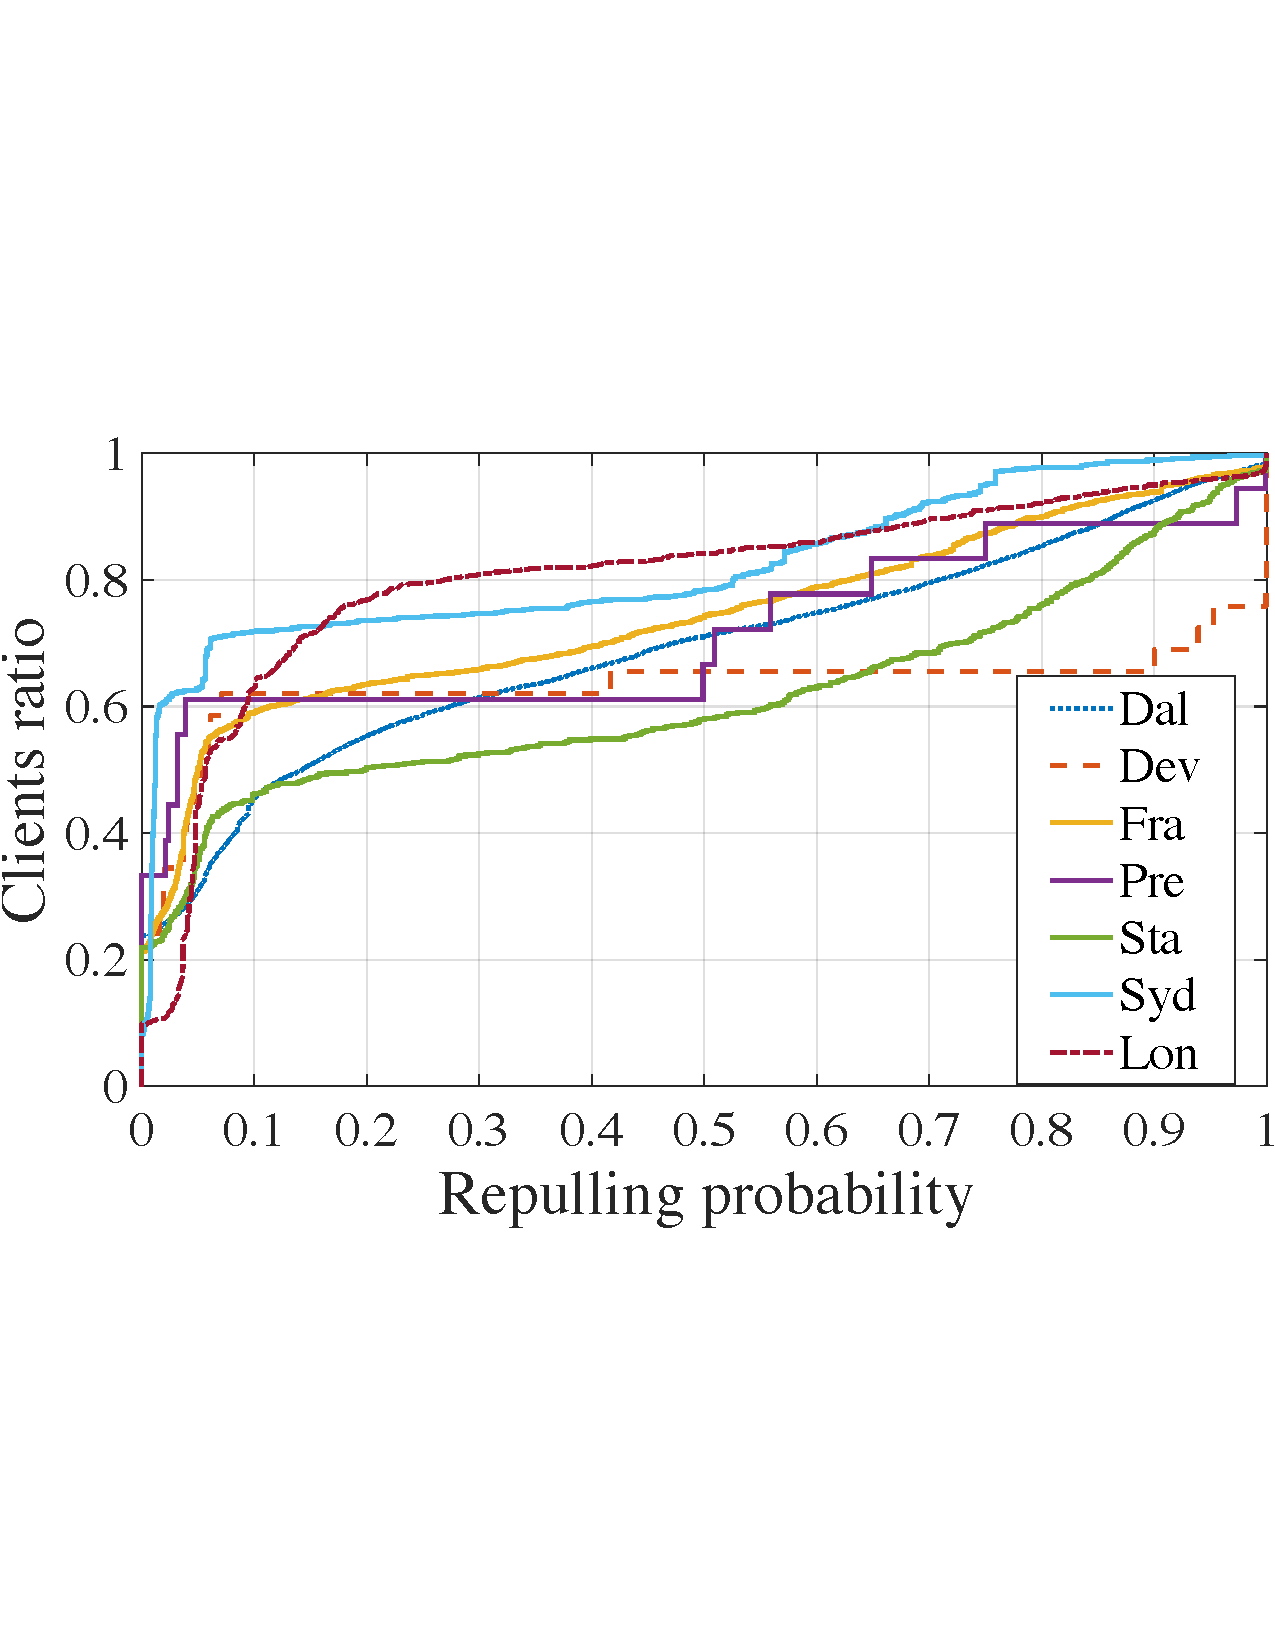
\includegraphics[width=0.9\textwidth]{graphs/cdf-client-repull-layer-request-ratio.pdf}
                \caption{CDF of Client repulling probability}% of LRU cache and preconstruct cache.}
                \label{fig:client-repull-cdf}
        \end{minipage}%
        \begin{minipage}{0.3\textwidth}
        \centering
        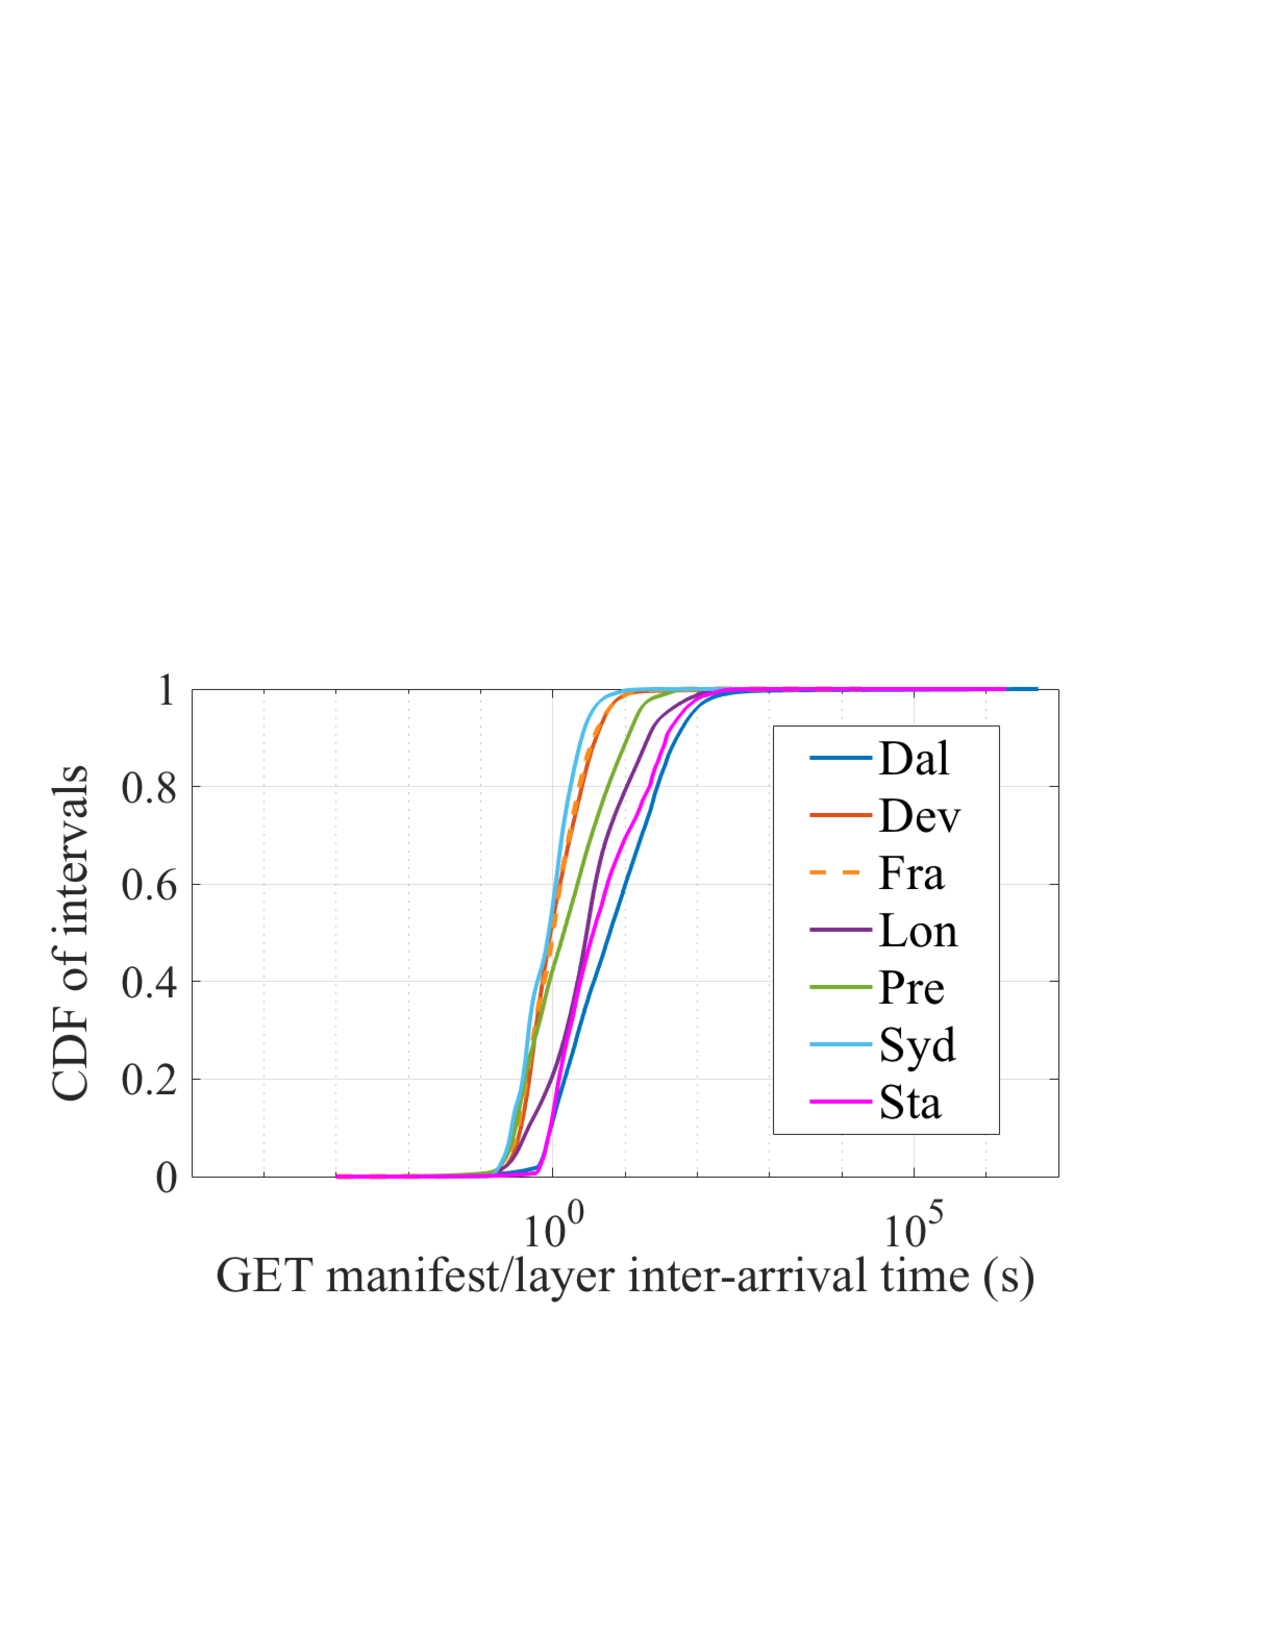
\includegraphics[width=0.9\textwidth]{graphs/GML-intervals.pdf}
        \caption{Intervals between \texttt{GET} manifest request and \texttt{GET} layer request}
        \label{fig:intervals}
   \end{minipage}
\end{figure*}





%\begin{figure}[!t]
%	\centering
%	\subfigure[CDF of compression ratio]{\label{fig_cdf_compression_ratio}
%		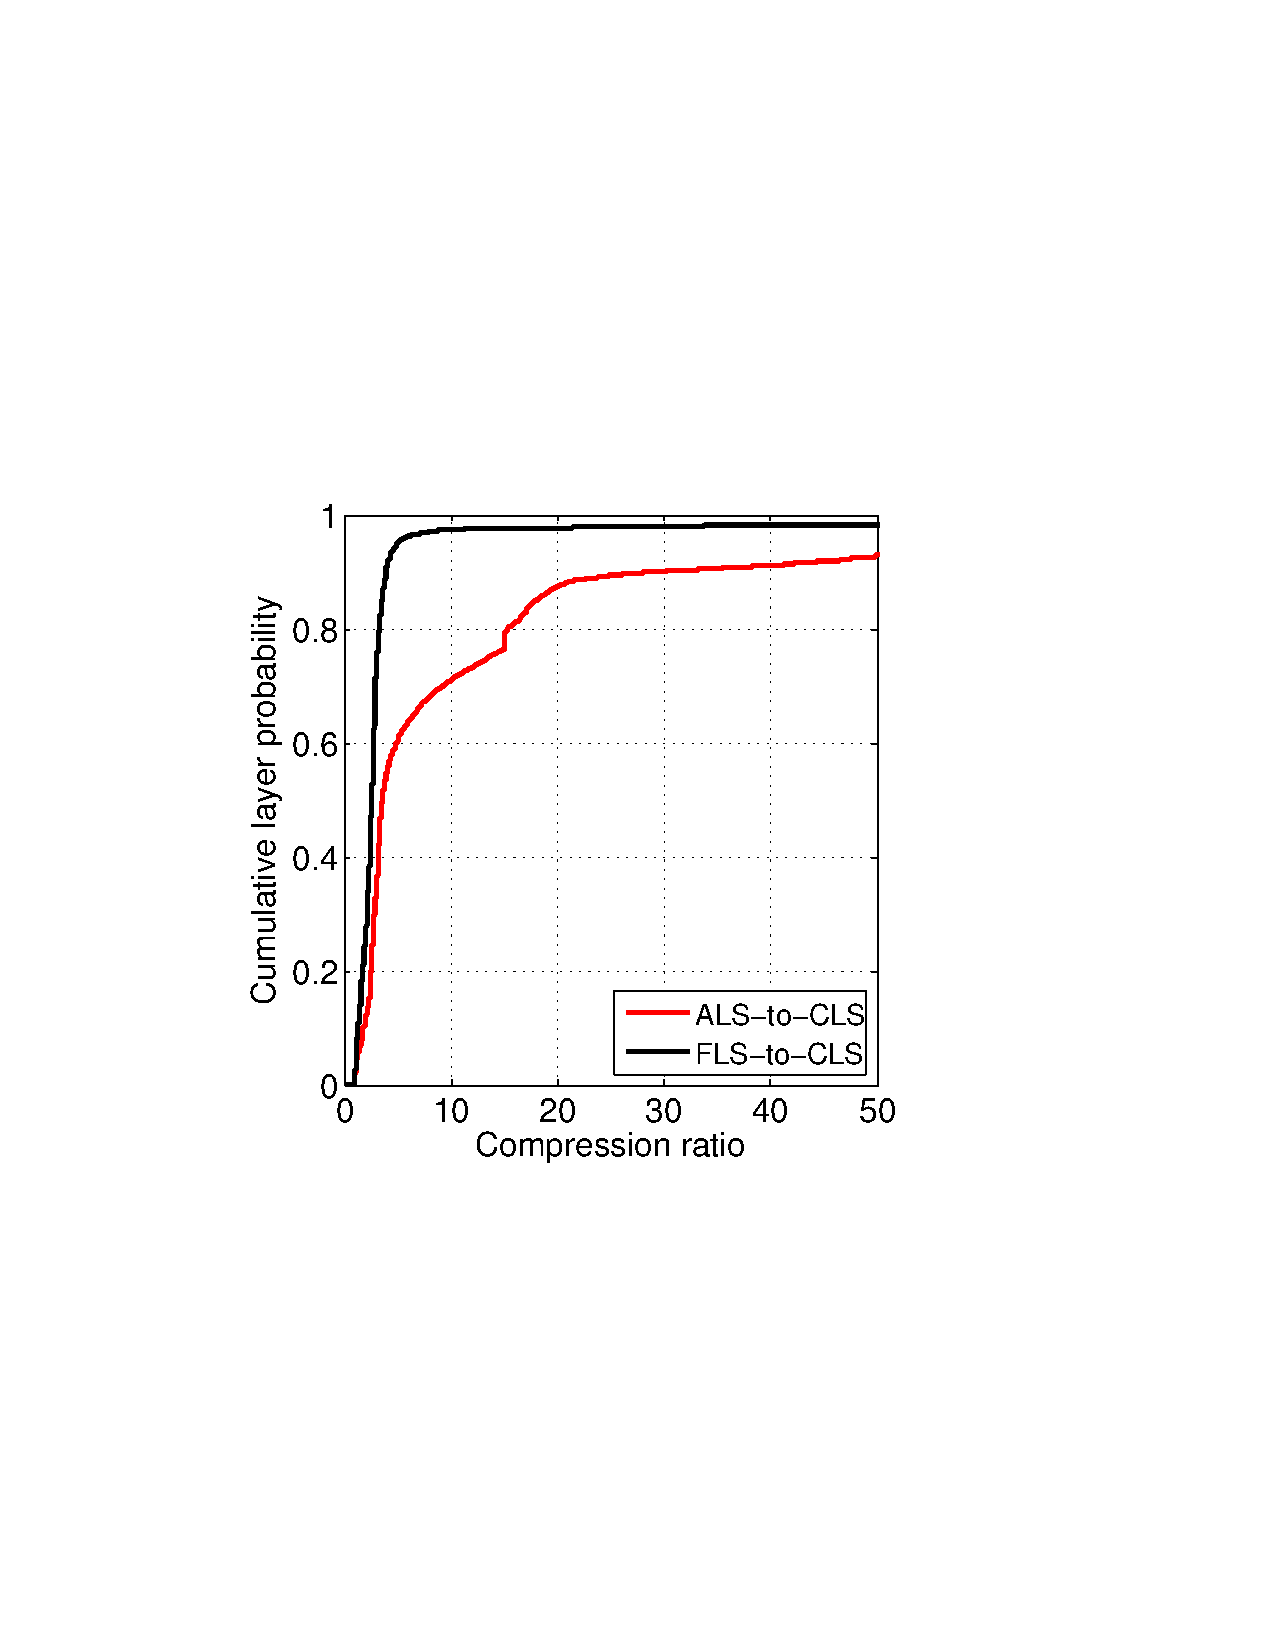
\includegraphics[width=0.23\textwidth]{graphs/cdf_compression_ratio.pdf}
%	}
%	\subfigure[Histogram of comp. ratios]{\label{fig_his_compression_ratio}
%		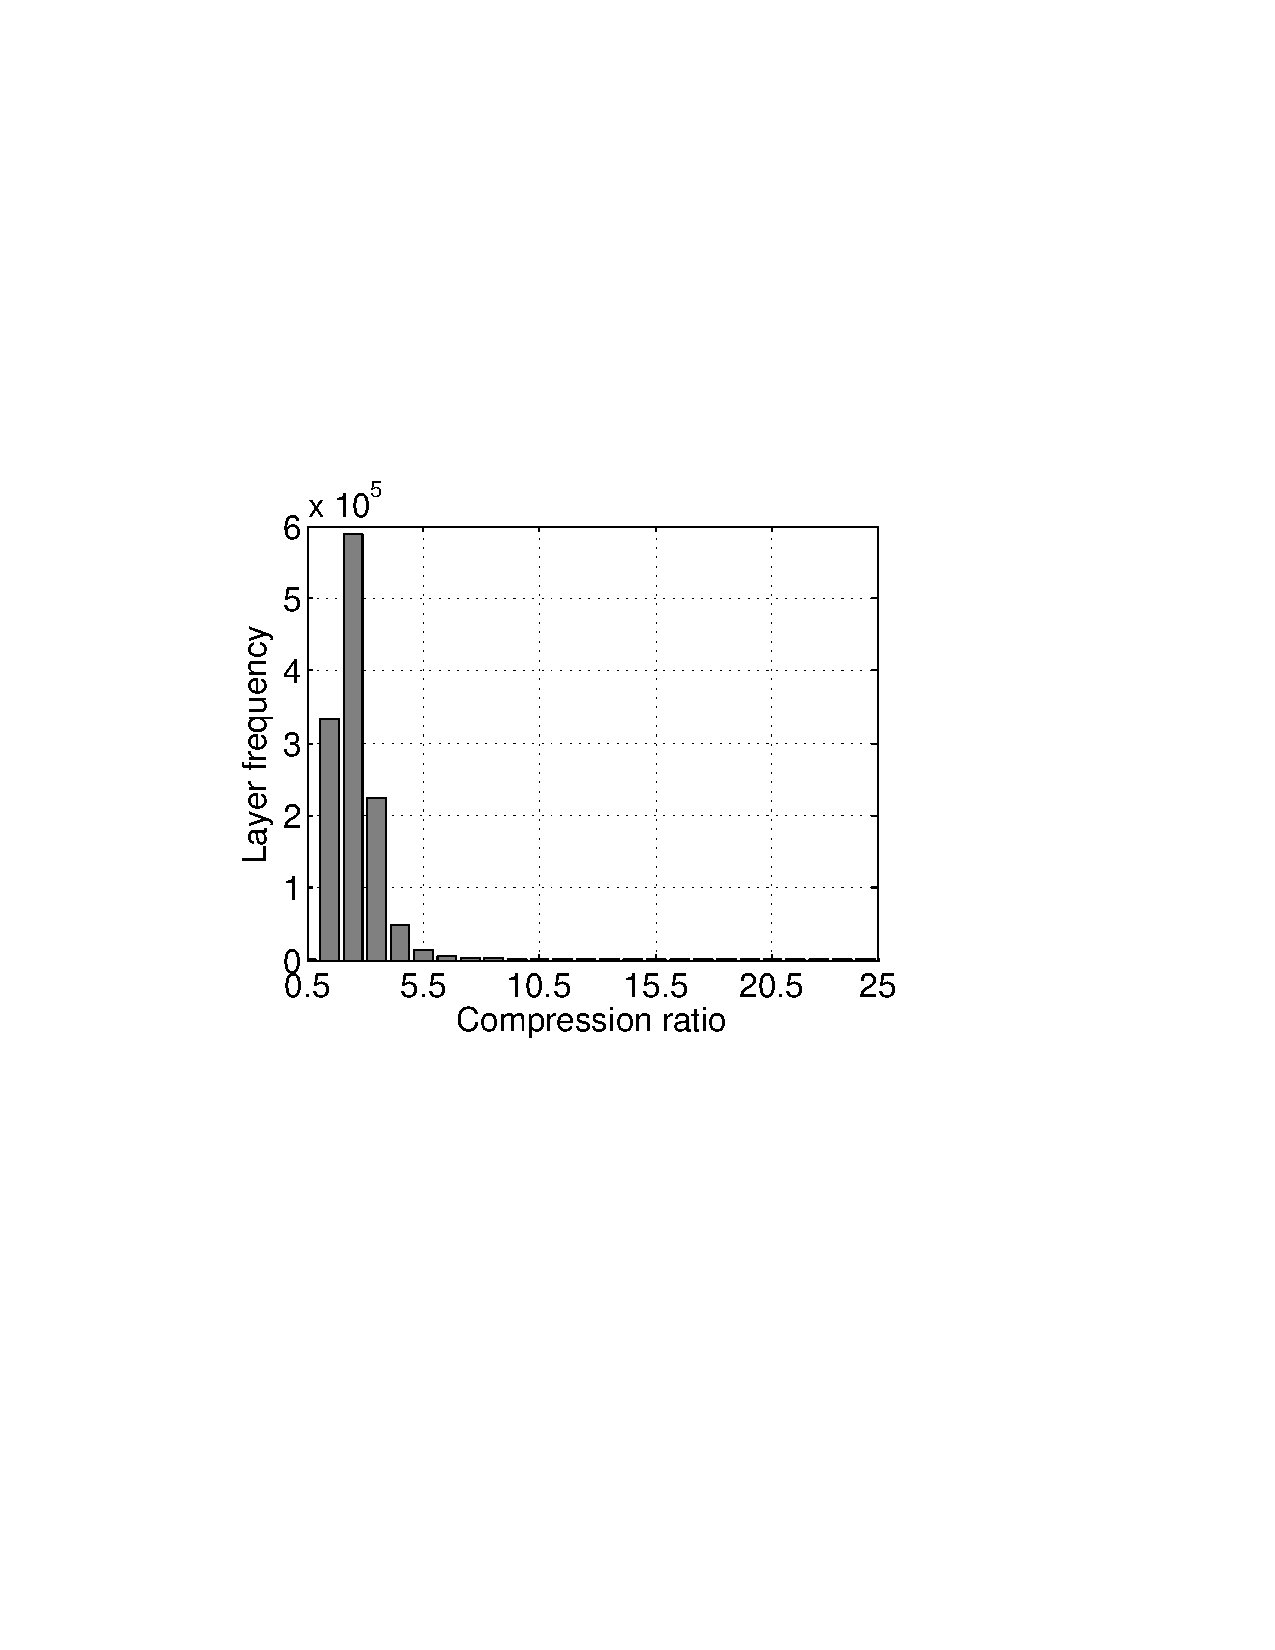
\includegraphics[width=0.223\textwidth]{graphs/his_compression_ratio.pdf}
%	}
%	\caption{Layer compression ratio distribution
%		%\vcomment{Different colors are used in figure (a) and (b) FLS/CLS\nancomment{will address later}}
%	}
%	\label{fig-compression-ratio}
%\end{figure}


%\begin{figure}[t]
%	\centering
%	\begin{minipage}{0.26\textwidth}
%		\centering
%		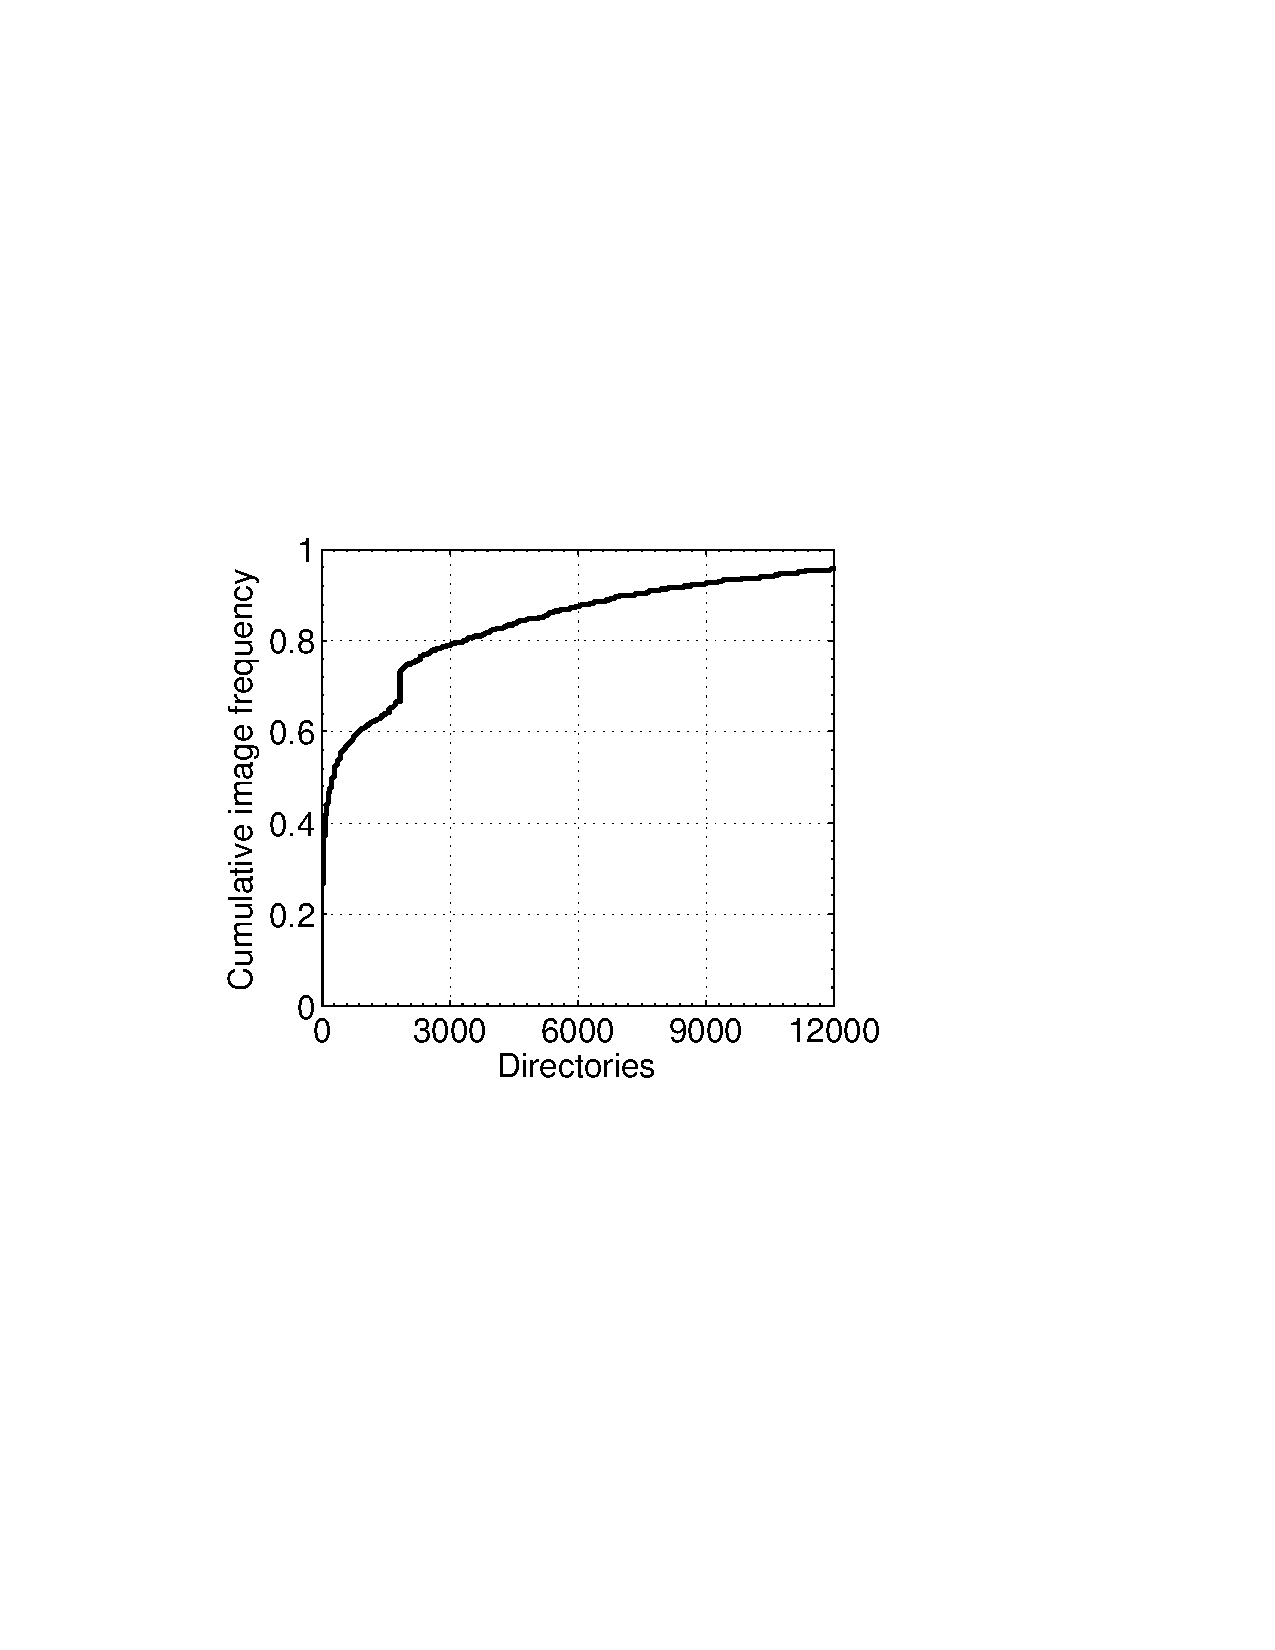
\includegraphics[width=1\textwidth]{graphs/dir.pdf}
%		\caption{CDF of images by\newline directories}
%		\label{fig-dir}
%	\end{minipage}%
%	\begin{minipage}{0.24\textwidth}
%		\centering
%		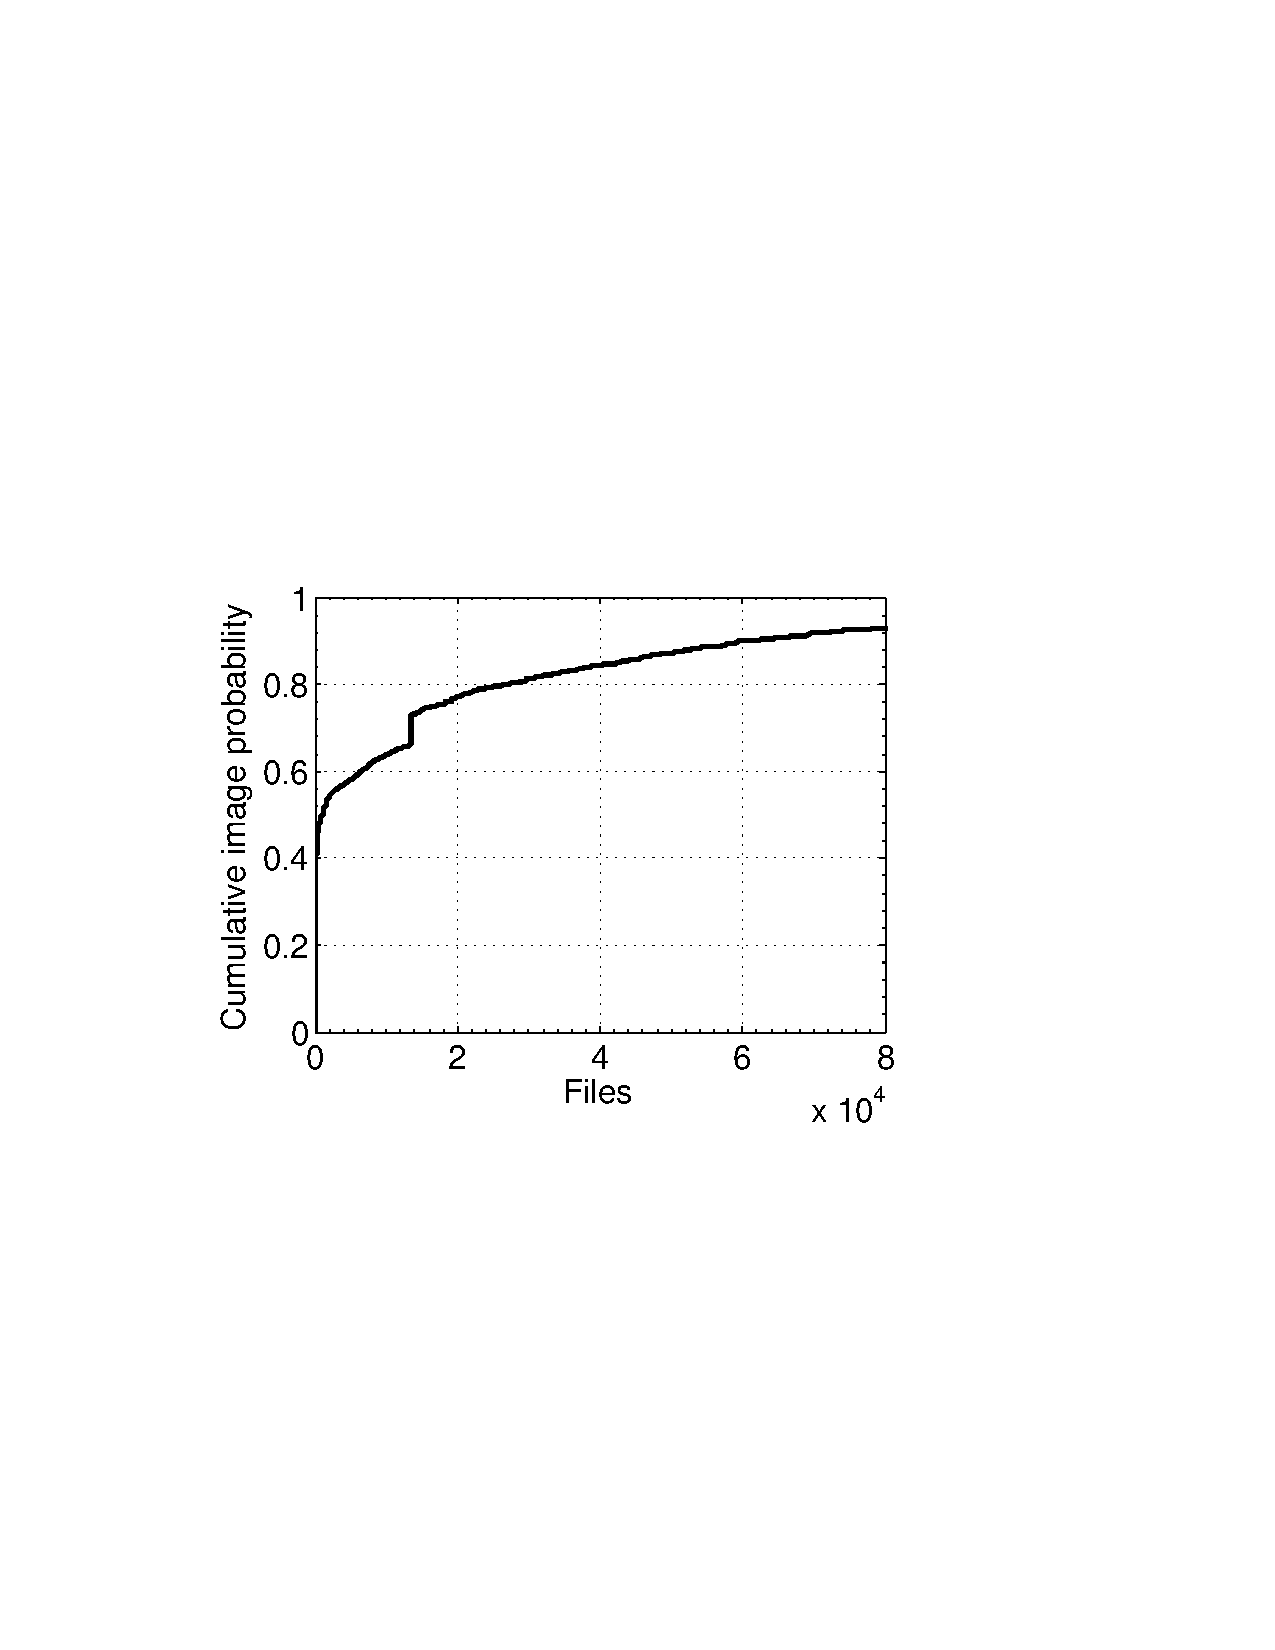
\includegraphics[width=1\textwidth]{graphs/file.pdf}
%		\caption{CDF of images by files}
%		\label{fig-file}
%	\end{minipage}
%\end{figure}

%\begin{figure}[htbp] 
%	\begin{minipage}{0.5\linewidth} 
%		\centering 
%		\includegraphics{circle} 
%		\caption{A Circle} 
%		\label{fig:circle} 
%	\end{minipage}% 
%	\begin{minipage}{0.5\linewidth} 
%		\centering 
%		\includegraphics{rectangle} 
%		\caption{A Rectangle} 
%		\label{fig:rectangle} 
%	\end{minipage} 
%\end{figure}

%
A promising approach to mitigate layer restoring overhead is predicting which layers will be accessed in the future and preconstructing them.
%
%To overcome the deduplication overhead, we analyze registry workloads
%and optimize the performance by exploring workload patterns and user
%access patterns.
%
%To study the feasibility of such a prediction approach, we analyze
%existing registry workloads from~\cite{dockerworkload}. %\todo{cite the workloads we studied here}.
%
We can exploit the fact that when a Docker client pulls an image
from the registry, it will first get the manifest of the
image, which includes references to the layers in the image.
%is metadata file of the image and contains a list of layers' digests.
%
%The client then parses the layer list in the manifests
%and compares it against a \emph{local layer index}.
%
%If a layer doesn't exist in the local layer index, the client will issue a \texttt{GET}
%request for this layer.
%
%Thus, to anticipate layer accesses, we can maintain a \emph{layer index} for each user
%at the registry to keep track of a user's access history and thereby determine which layer
%will be requested by the user after the \texttt{GET} manifest request.
%
However, the client might or might not follow up with layer \texttt{GET} requests.
%
Further, there might be not enough time to reconstruct the layer
between the manifest and layer \texttt{GET}s.


\paragraphQ{Do clients issue repeated GETs}
%
Typically, if a layer is already stored locally, then the client will not
fetch this layer again.
%
However, higher level container orchestrators, e.g., Kubernetes, allow users to configure different policies
for starting new containers. Kubernetes, e.g., allows policies such as
\texttt{IfNotPresent}, i.e,  only get the layer if not present, or \texttt{AlwaysGet}, i.e.
retrieve the layer, even if it is already present locally.
%
This fact needs to be considered when predicting whether a layer will
be pulled by a user or not.

We use the IBM Cloud registry workload~\cite{dockerworkload} to analyze the likelihood for
a user to \emph{repull} an already present layer.
%
The traces span $\sim$80 days for 7 different registry clusters:
\texttt{Syd} (Sydney), \texttt{Dal} (Dallas), \texttt{Fra} (Frankfurt), \texttt{Lon} (London),
\texttt{Dev} (Development), \texttt{Pre} (Prestaging), and \texttt{Sta} (Staging).
%
Figure~\ref{fig:layer-repull-cdf} shows the
CDF of layer \texttt{GET} counts by the same clients. 
%
The analysis shows that the majority of layers are only fetched once by the same clients.
%For example, 97\% of layers from \texttt{Syd} are only fetched once by the same clients.
%
However, there are clients, which repull the same layers continuously.  For
example, a client from \texttt{Lon} fetched the same layer 19,300 times.
%When different clients \texttt{pull} the same repository, they will fetch
%different amount of layers from the repository based on the contents of their
%local layer dataset.  The local layers can vary with time due to clearing of
%the data so the same clients can fetch different amounts of layers at
%different times.  Therefore, a \texttt{pull manifest} request doesn't usually
%result in repulling all the layers in the repository.  Here, we define
%\emph{repulling a repository} as repulling the layers in the repository for
%the same client.  Figure~\ref{fig:repo-repull-cdf} shows the CDF of the
%probability of repository repulling, calculated as the number of \texttt{pull
%manifest} resulting in repository repulling divided by the total number of
%\texttt{pull manifest} requests issued for the same repository.  We see that
%majority of repositories aren't repulled.  The percentage of repositories
%whose repull probability is zero (i.e. are pulled only once by a client)
%ranges from 57\% for \texttt{Prestage} to 85\% for \texttt{Syd}.  Only 20\% of
%repositories from  \texttt{Prestage}, \texttt{Stage}, and \texttt{Syd} have a
%repulling probability higher than 0.5.  We also observe that few repositories'
%repulling probability is 1, indicating repulls everytime by the clients.

%
%\LR{Need to make sure that the following is not repeated in 4.4 (Caching Layers)}
%\NZ{its duplicated}
%We define \emph{repulling} as the act of fetching the same layer more than once
%by the same user.
% before because they are no longer present on the user side.
Figure~\ref{fig:client-repull-cdf} shows the corresponding client repull probability,
calculated as the number of repulled layers divided by the
number of total \texttt{GET} layer requests issued by the same client.
%
We see that 50\% of the clients have a repull probability of less than 0.2
across all registries.
%
We also observe that the slope of the CDFs is steep at both lower and higher probabilities
but becomes flat in the middle.
%
This suggests that we can split clients into two classes, always-pull clients
and pull-once clients, e.g., based on a threshold.
%
%Thus, to determine whether a client will \texttt{repull} a layer or not, we
%can compute the client repull probability and place the client in one of these classes.
%
%significant amount of clients have a low repulling proability.
%
%For example, 71\% of clients from \texttt{syd} have a repulling probability lower
%than 0.1.
%
%Very few clients have a high repulling probability.  For instance,
%only 2\% clients have a repulling probability higher than 0.9 from
%\texttt{Dal}.


%We also observe that the slope is steep at both lower and higher probabilities.
%However, the slope becomes flat in the middle.
%
%For example, the slope at probabilities between 0.1 and 0.9 for \texttt{dev}
%almost equals to zero.
%
%In this case, the high repulling probability clients can be classified as
%always-pull clients, and the low repulling probability clients as pull-once
%clients.
%
%The few clients in the middle are considered as \emph{erratic}.
%
%Thus, to determine whether a client will \texttt{repull} a layer or not, we
%consider the client repulling probability and the layer repull count.
%From the probability distribution of the clients repulling, we can observe
%that a significant chunk of the clients have very low repulling probability
%and another chunk of the clients have a very high repulling probability, with
%few clients in the middle. For simplicity of implementation, the high
%probability clients can be classified as always repulling clients, and the low
%probability clients as never repulling (i.e. they pull only once). The few
%clients in the middle are considered as \emph{erratic} and no classification
%is made for them.


%\begin{figure*}[t]
%		\begin{minipage}{0.32\linewidth}
%			\centering
%			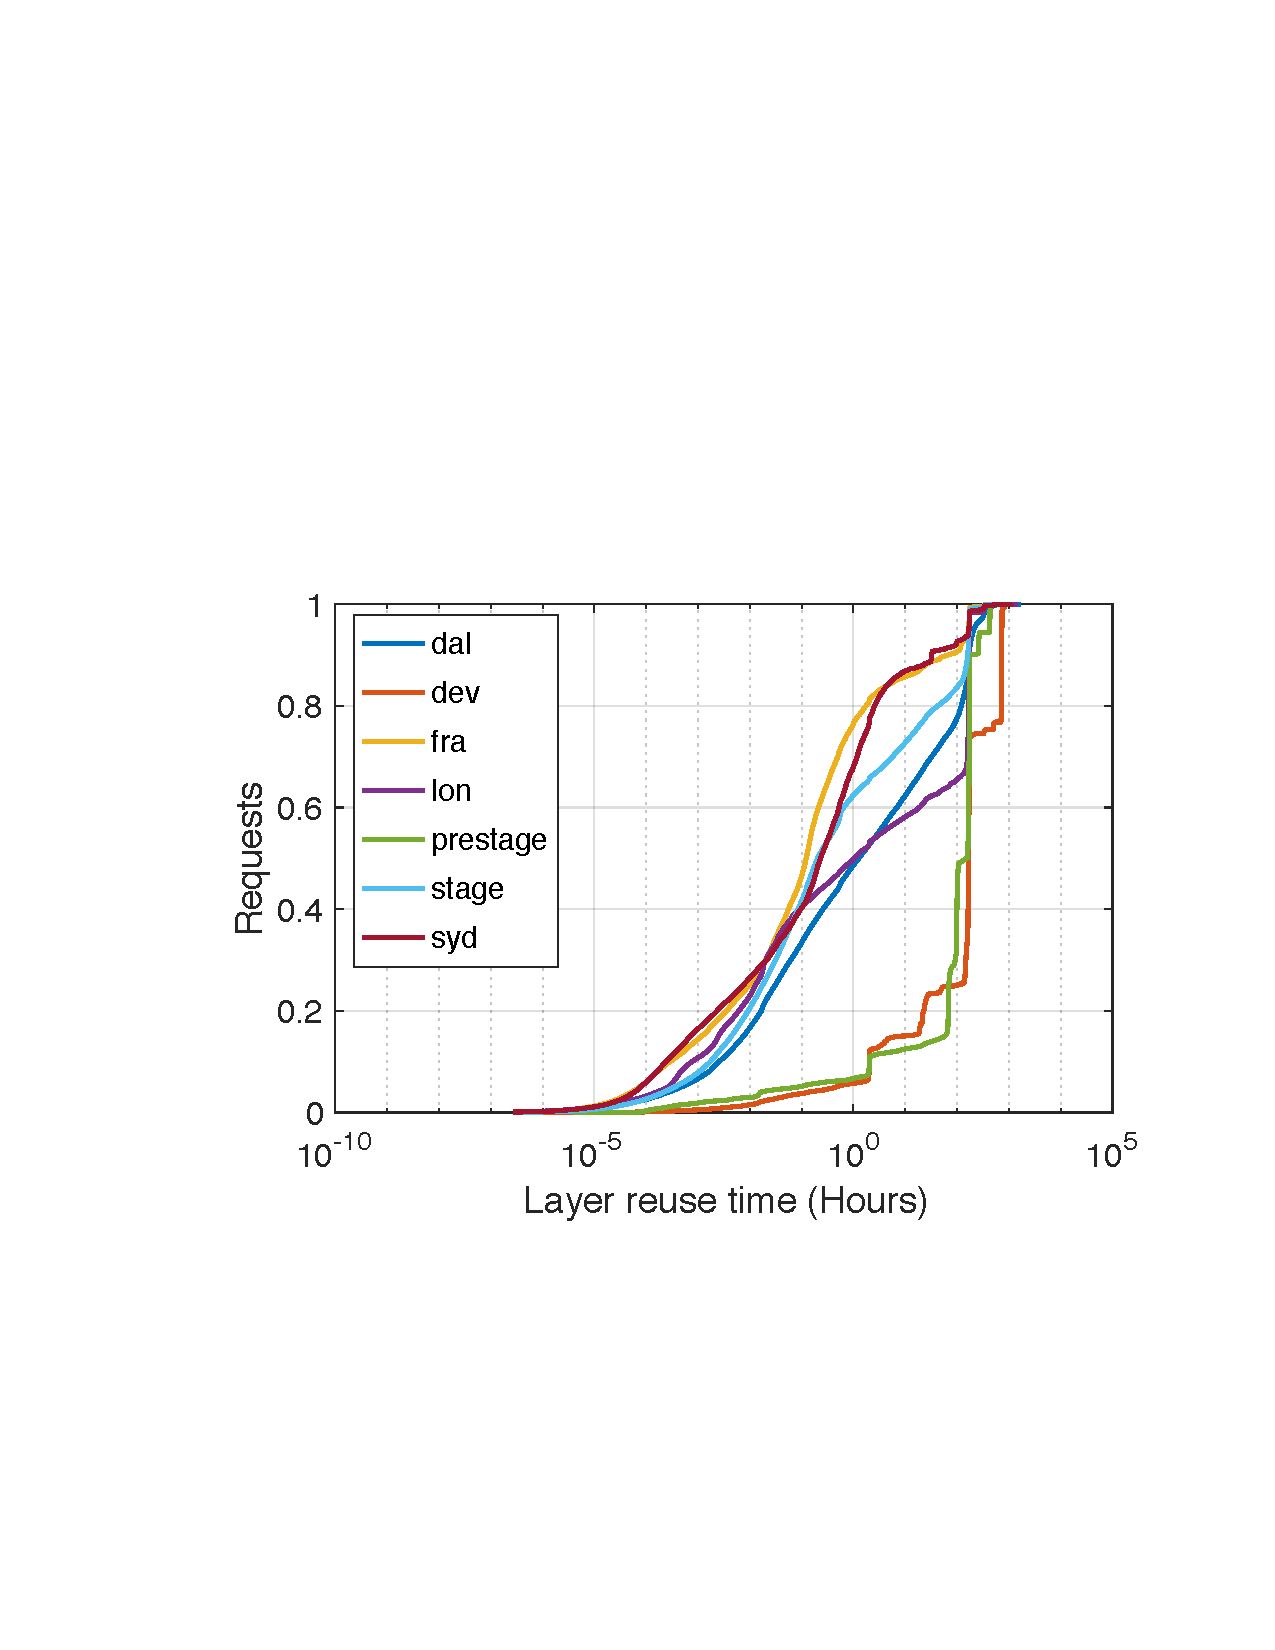
\includegraphics[width=1\textwidth]{graphs/layer-reusetime.pdf}
%		%	\caption{CDF of layer reuse time.}
%		%	\vspace{-3pt}
%			\label{fig:layer-reuse}
%		\end{minipage}
%			\begin{minipage}{0.32\linewidth}
%				\centering
%				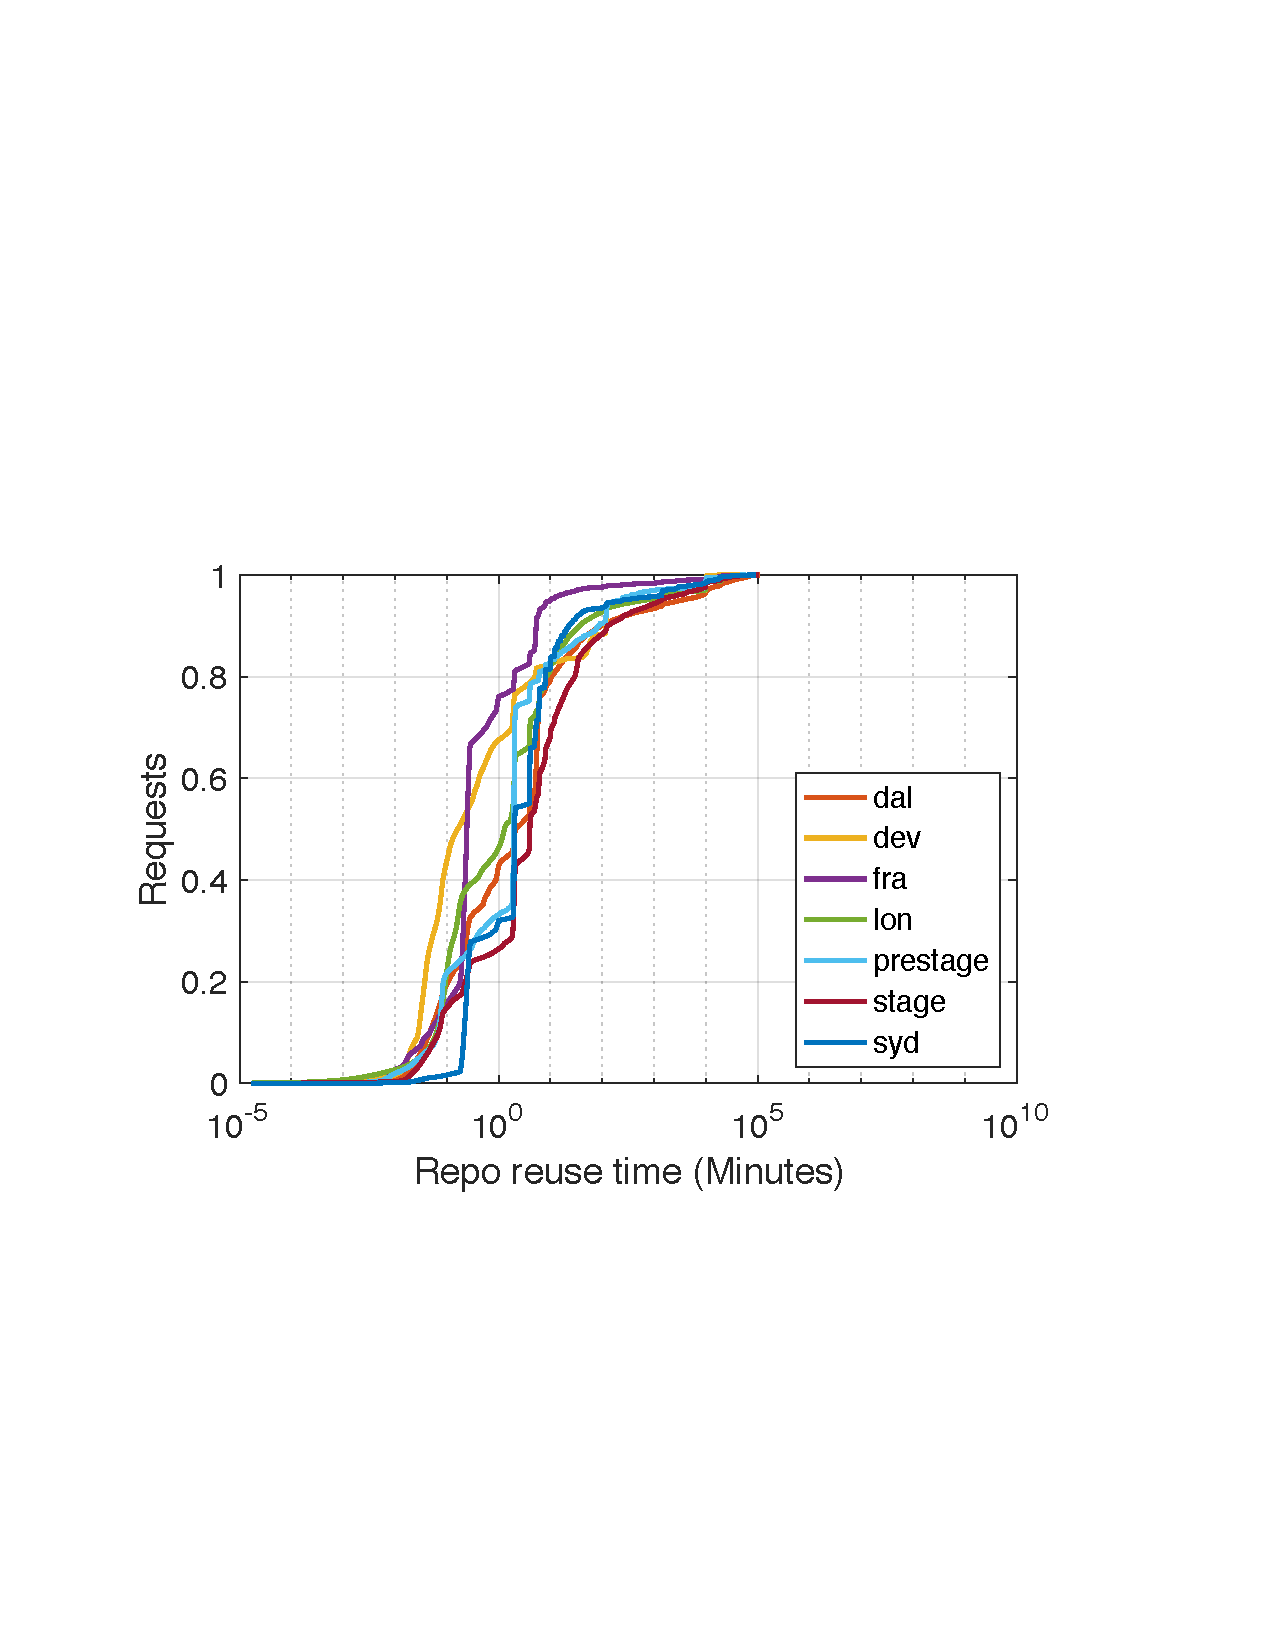
\includegraphics[width=1\textwidth]{graphs/repo-reusetime.pdf}
%			%	\caption{PDF of repository reuse time.}
%				%	\vspace{-3pt}
%				\label{fig:repo-reuse}
%			\end{minipage}
%		\begin{minipage}{0.32\linewidth}
%			\centering
%			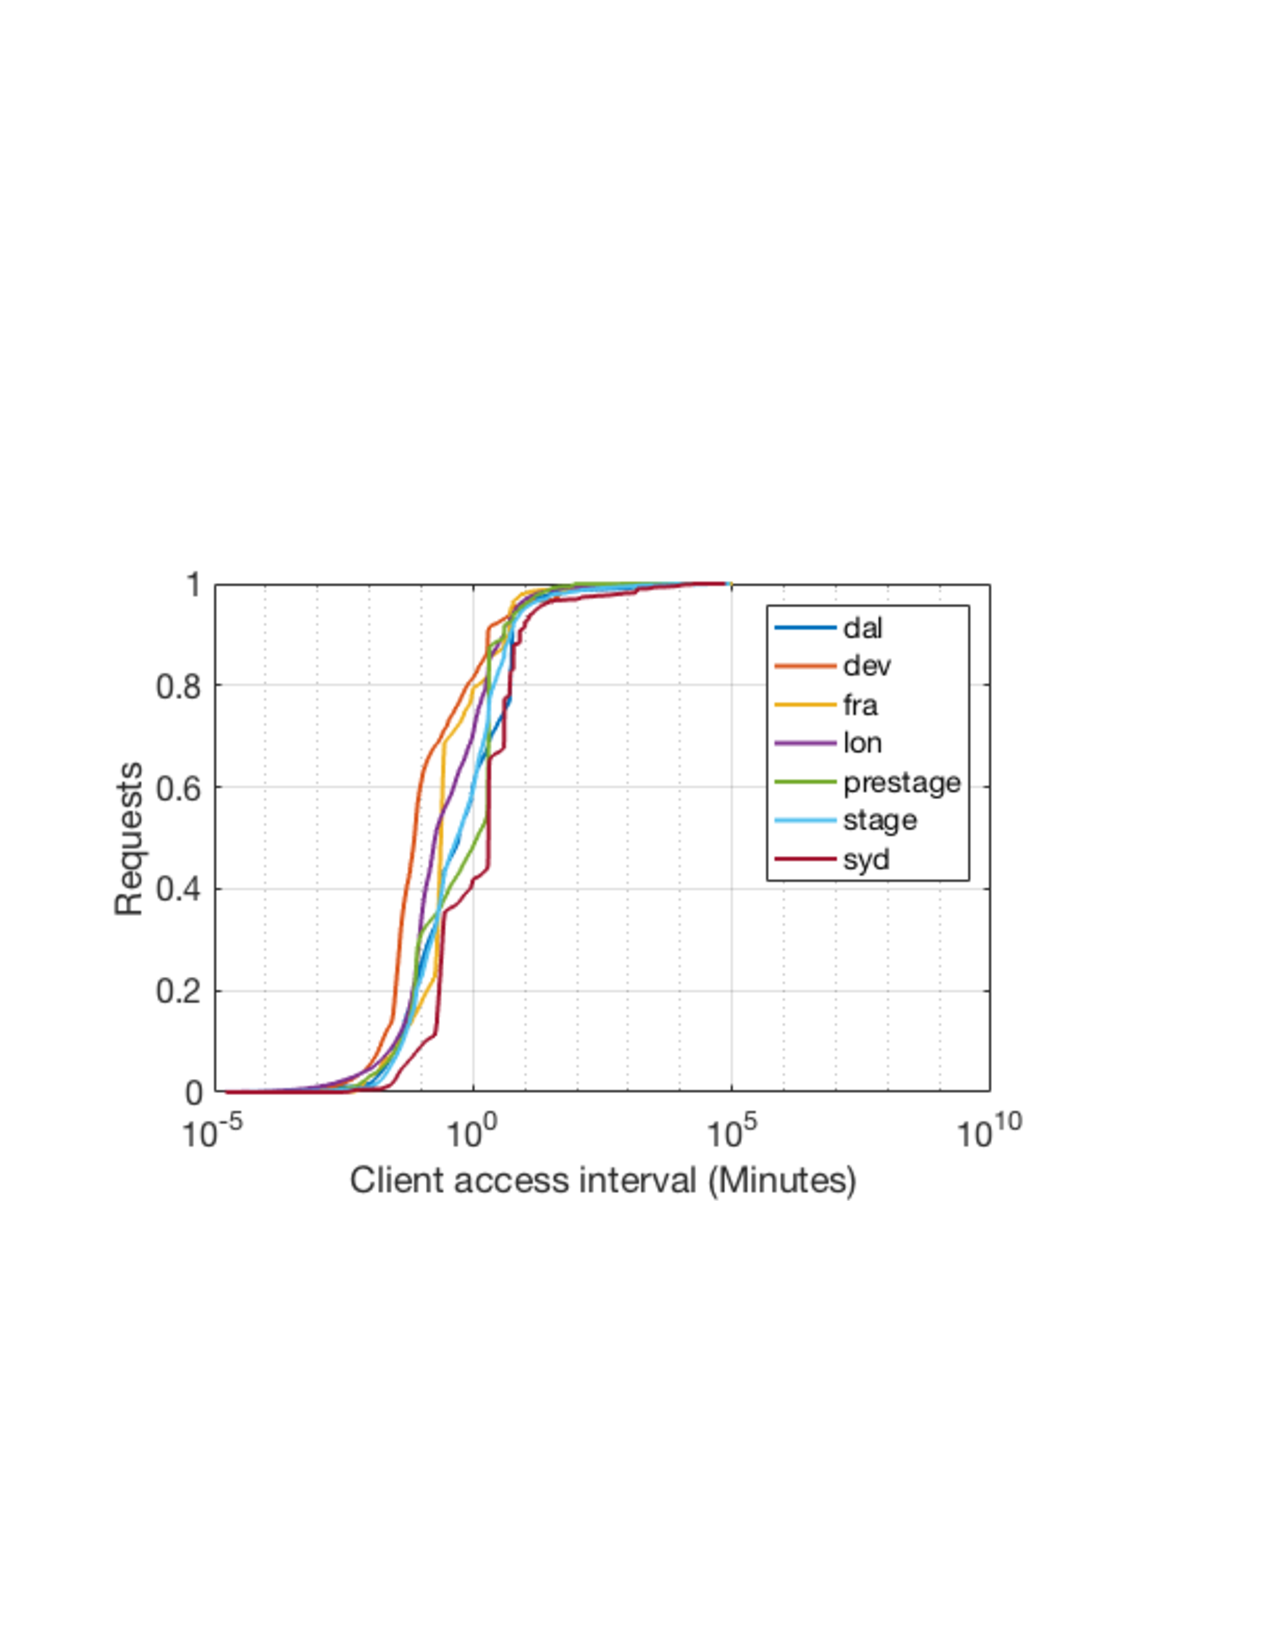
\includegraphics[width=1\textwidth]{graphs/user-intervals.pdf}
%			%\caption{PDF of client access intervals.}
%			%	\vspace{-3pt}
%			\label{fig:user-interval}
%		\end{minipage}
%	\caption{CDF of reusetime for layers, repositories and clients' access intervals.}
%	\label{fig:layer-reuse}
%\end{figure*}
\begin{figure}[t]
	\centering
	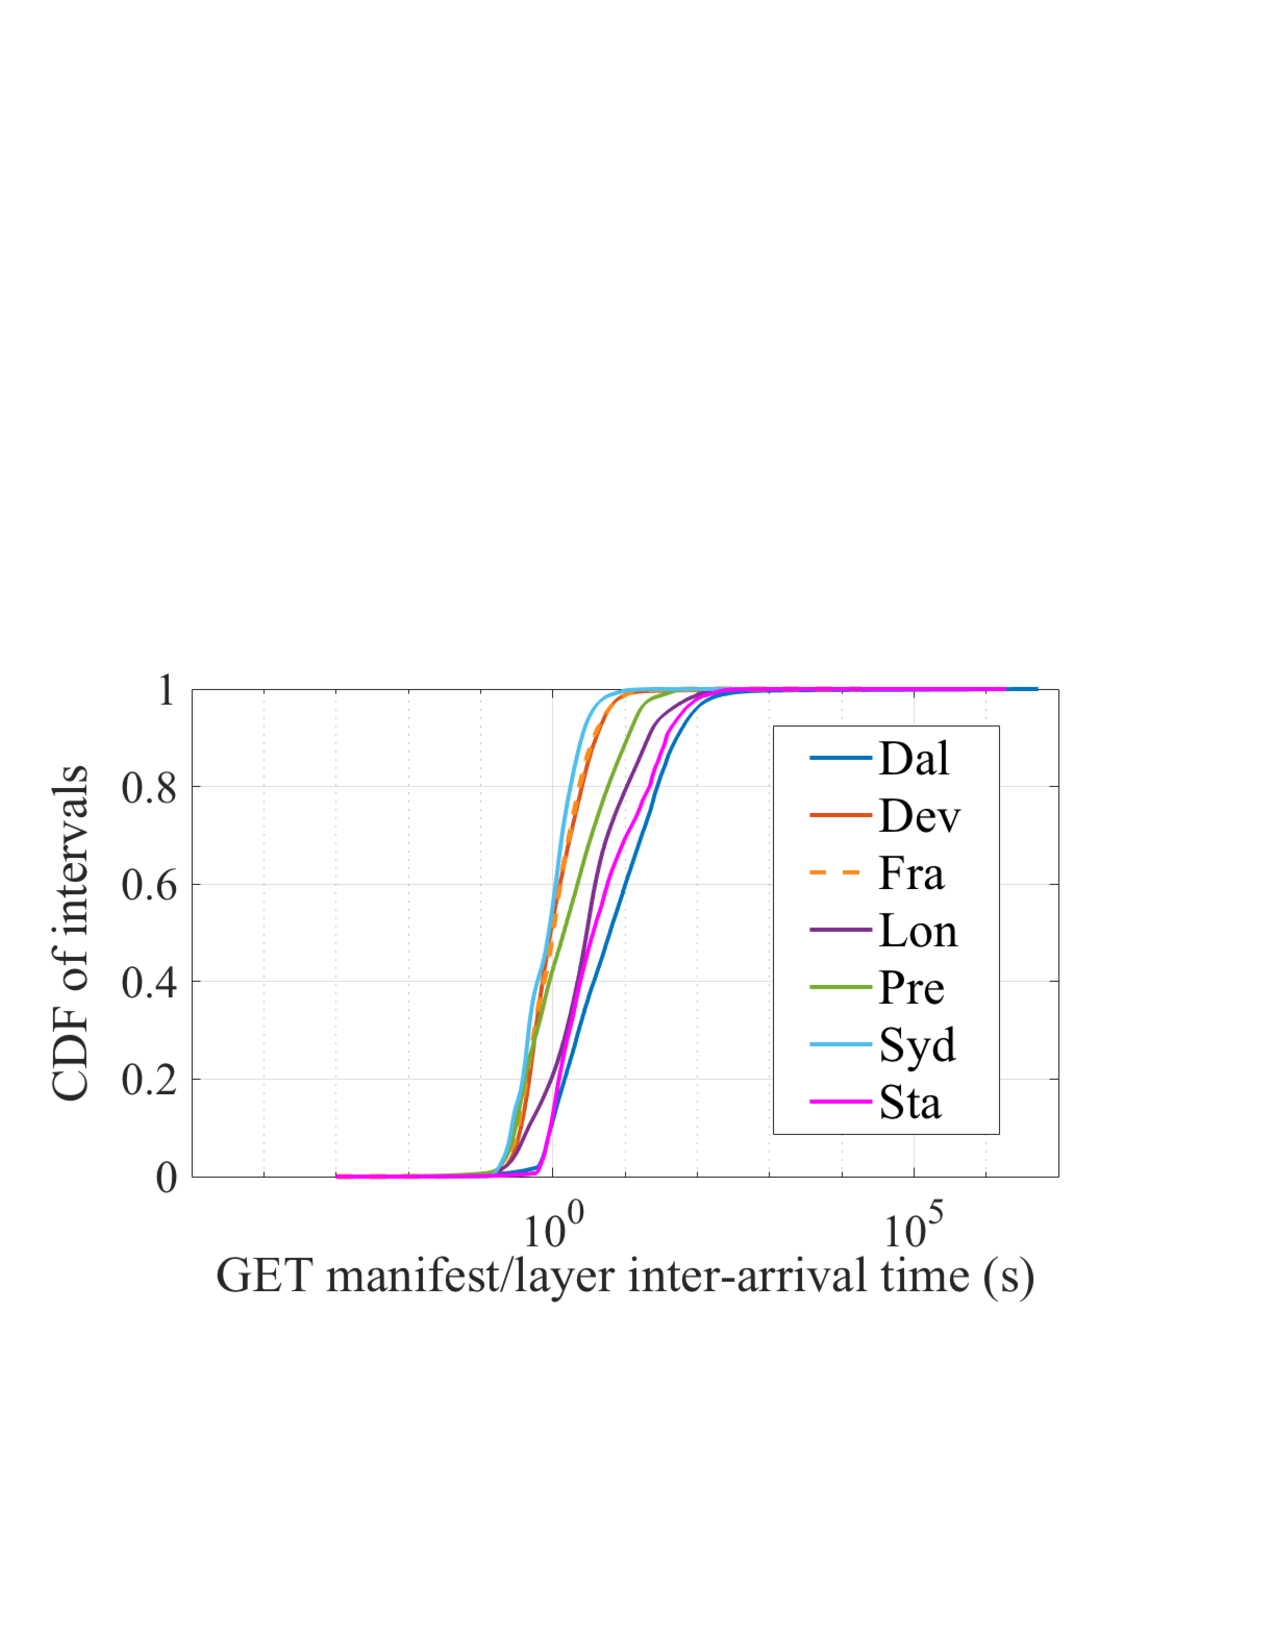
\includegraphics[width=0.3\textwidth]{graphs/GML-intervals.pdf}
	\caption{Intervals between \texttt{pull} manifest request and \texttt{pull} layer request}
	%	\vspace{-3pt}
	\label{fig:intervals}
	
\end{figure}
%\begin{figure*}[!t]
%	\centering
%	\subfigure[Layer repull count]{
%		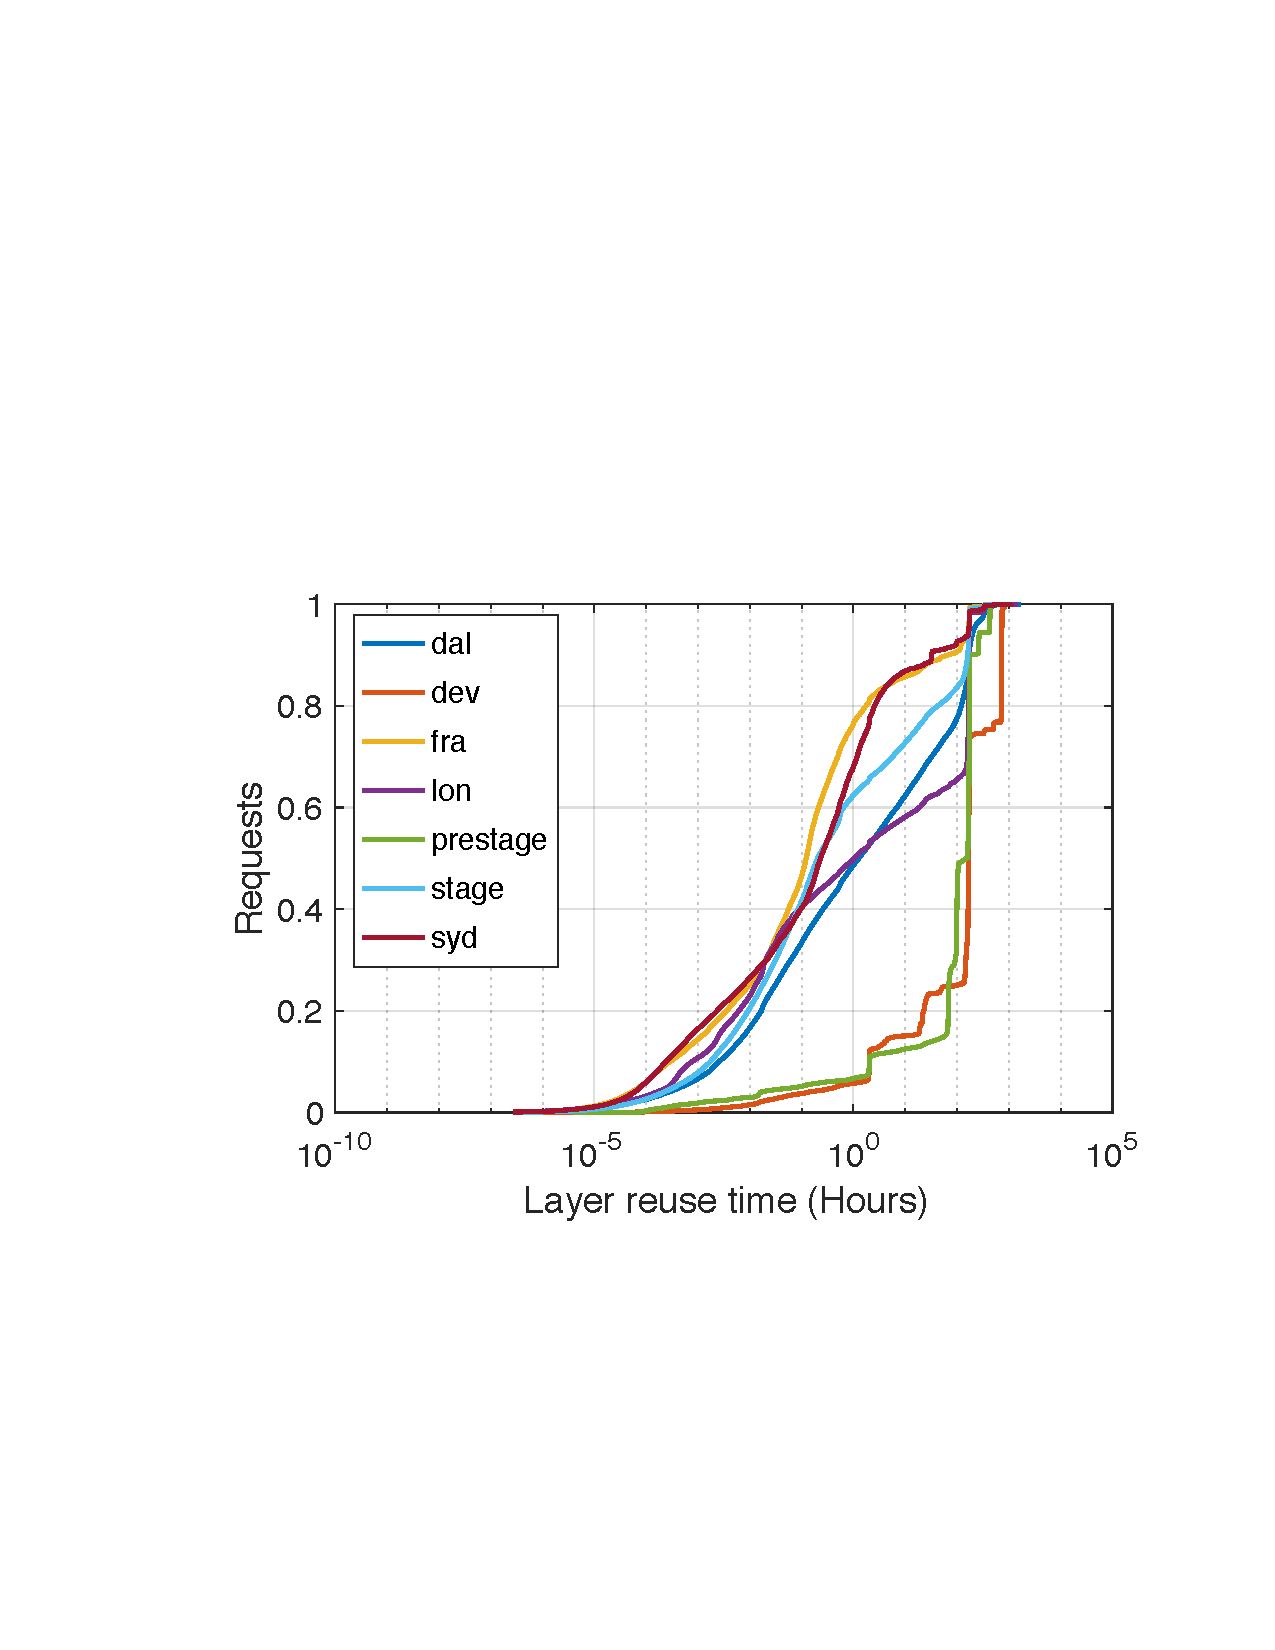
\includegraphics[width=0.2\linewidth]{graphs/layer-reusetime.pdf}
%			\label{fig:layer-reuse}
%	}
%	\subfigure[Repository repulling probability]{
%		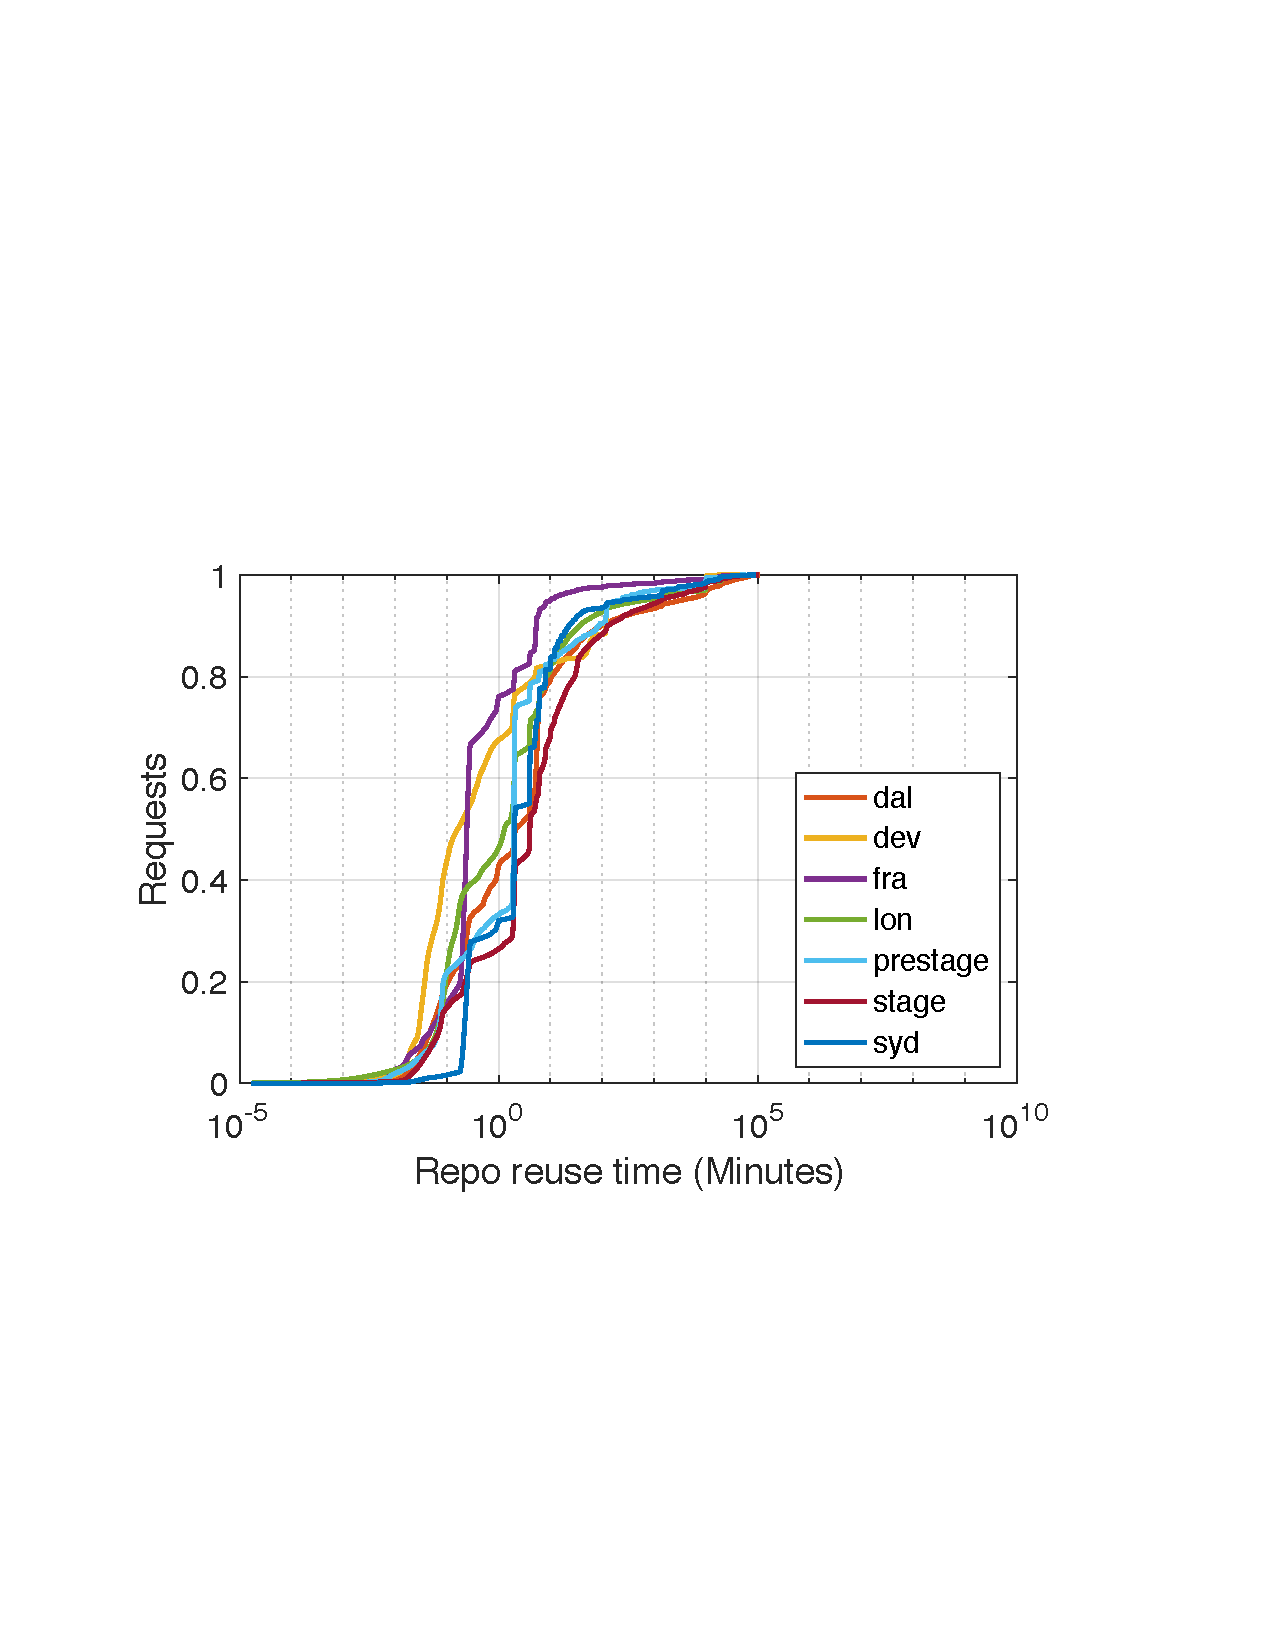
\includegraphics[width=0.2\linewidth]{graphs/repo-reusetime.pdf}
%				\label{fig:repo-reuse}
%	}
%	\subfigure[Client repulling probability]{
%		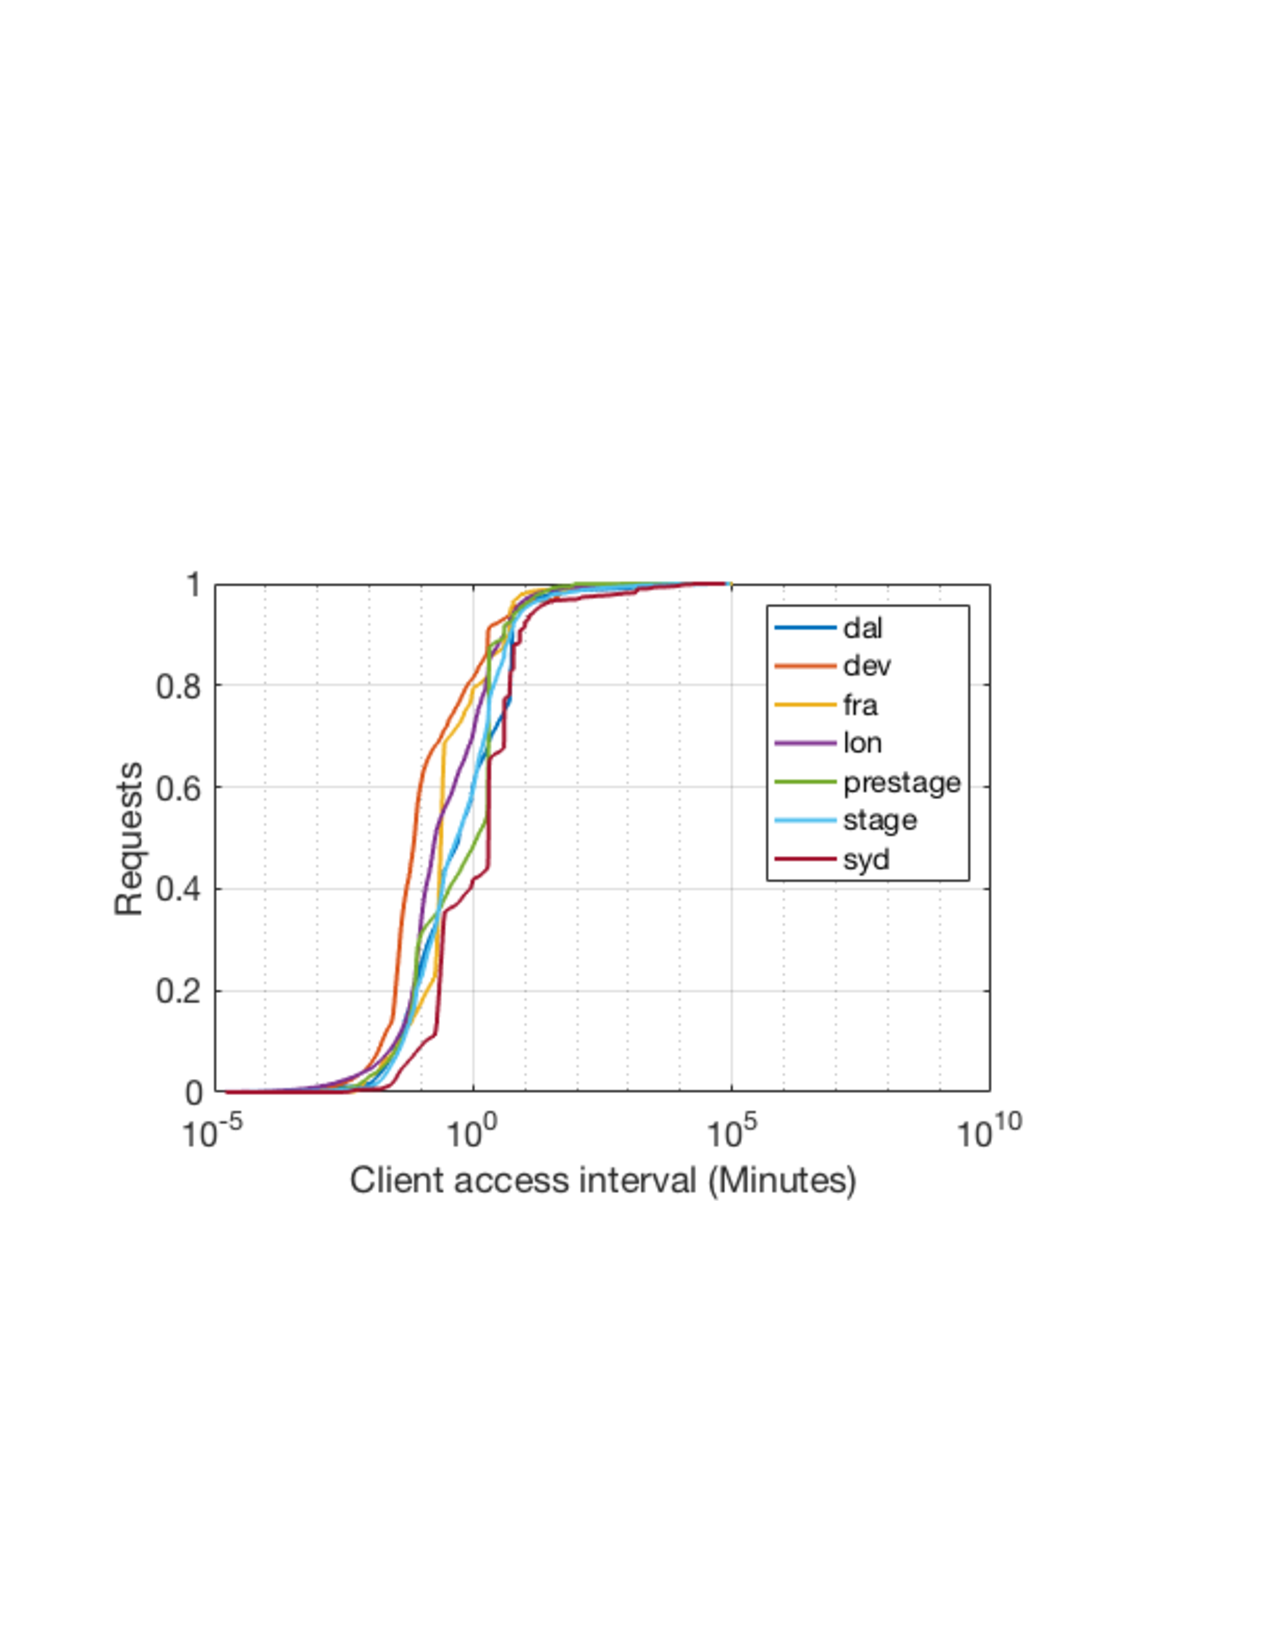
\includegraphics[width=0.2\linewidth]{graphs/user-intervals.pdf}
%			\label{fig:user-interval}
%	}
%	\caption{CDF of reusetime for layers, repositories and clients' access intervals.}
%	\label{fig:fig-reuse}
%\end{figure*}

%\begin{figure}[t]
%	\centering
%	\begin{minipage}{0.26\textwidth}
%		\centering
%		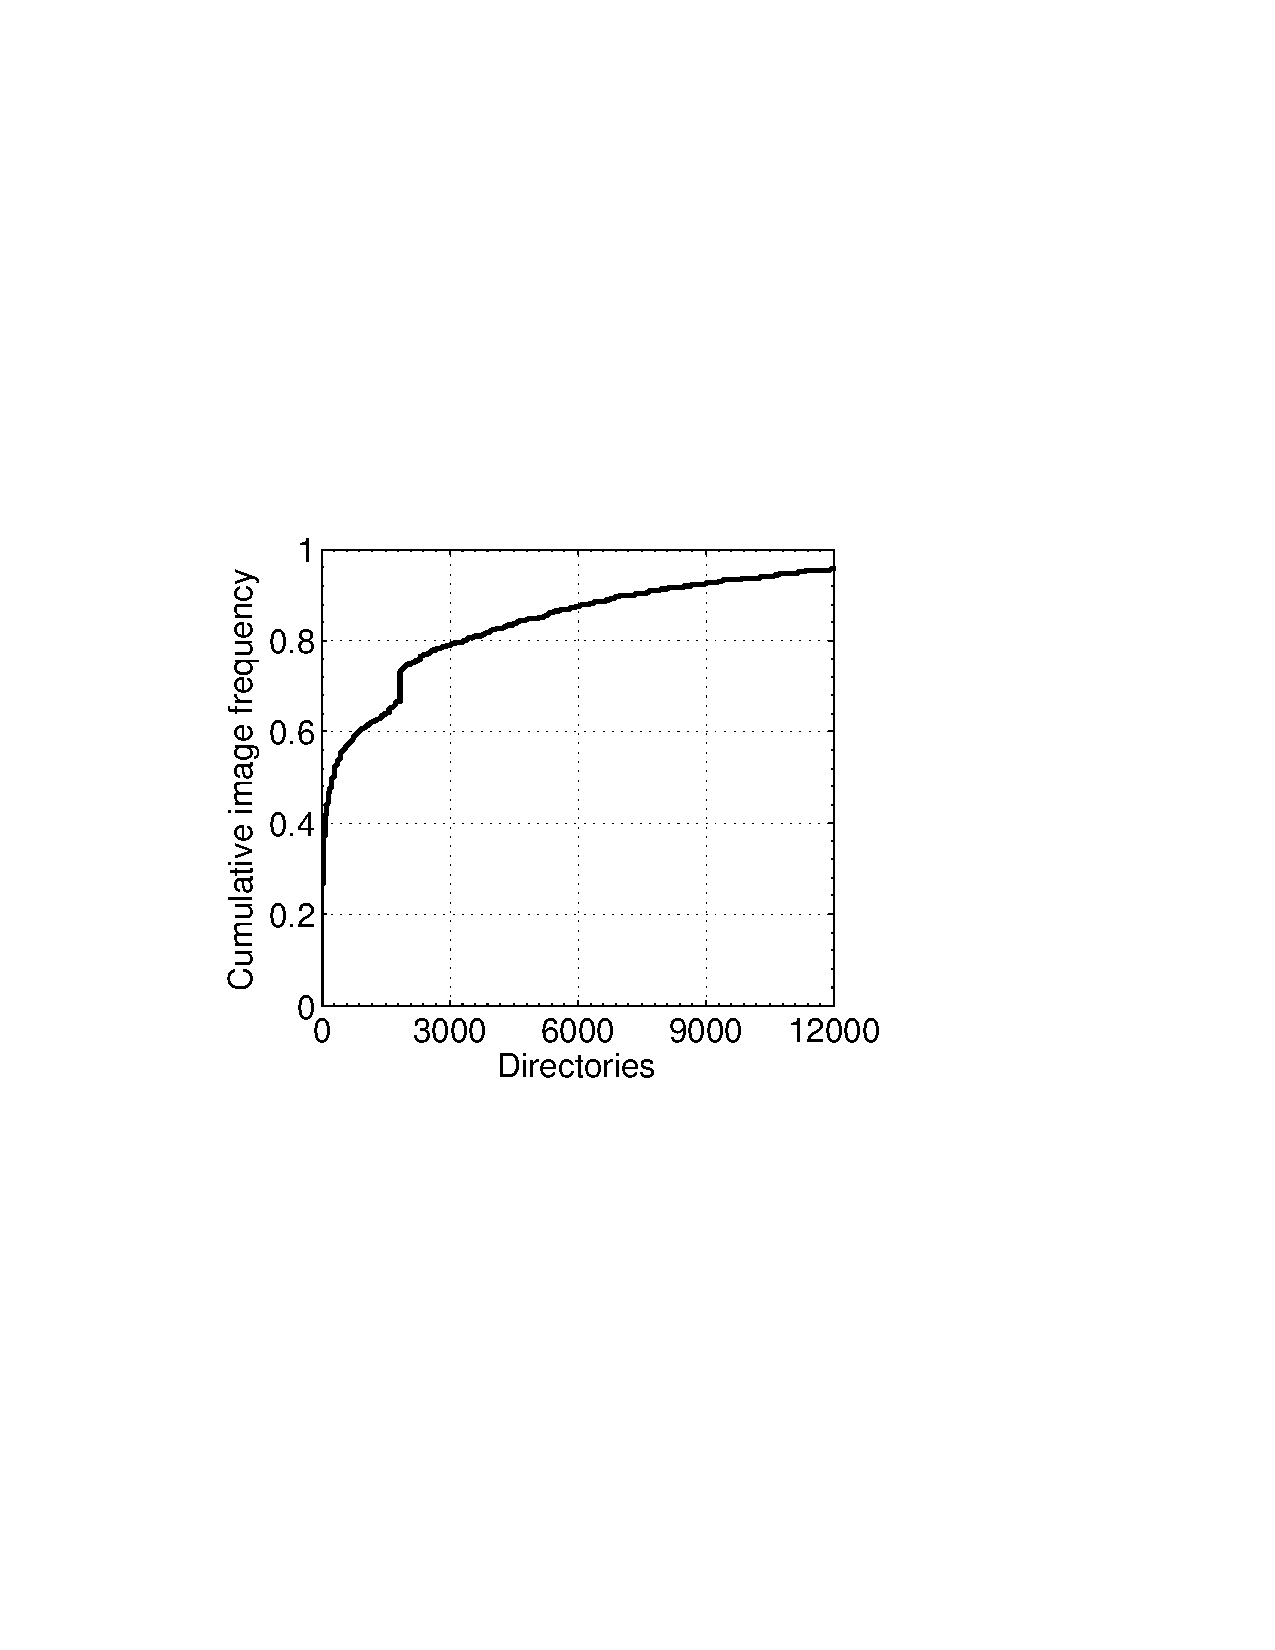
\includegraphics[width=1\textwidth]{graphs/dir.pdf}
%		\caption{CDF of images by\newline directories}
%		\label{fig-dir}
%	\end{minipage}%
%	\begin{minipage}{0.24\textwidth}
%		\centering
%		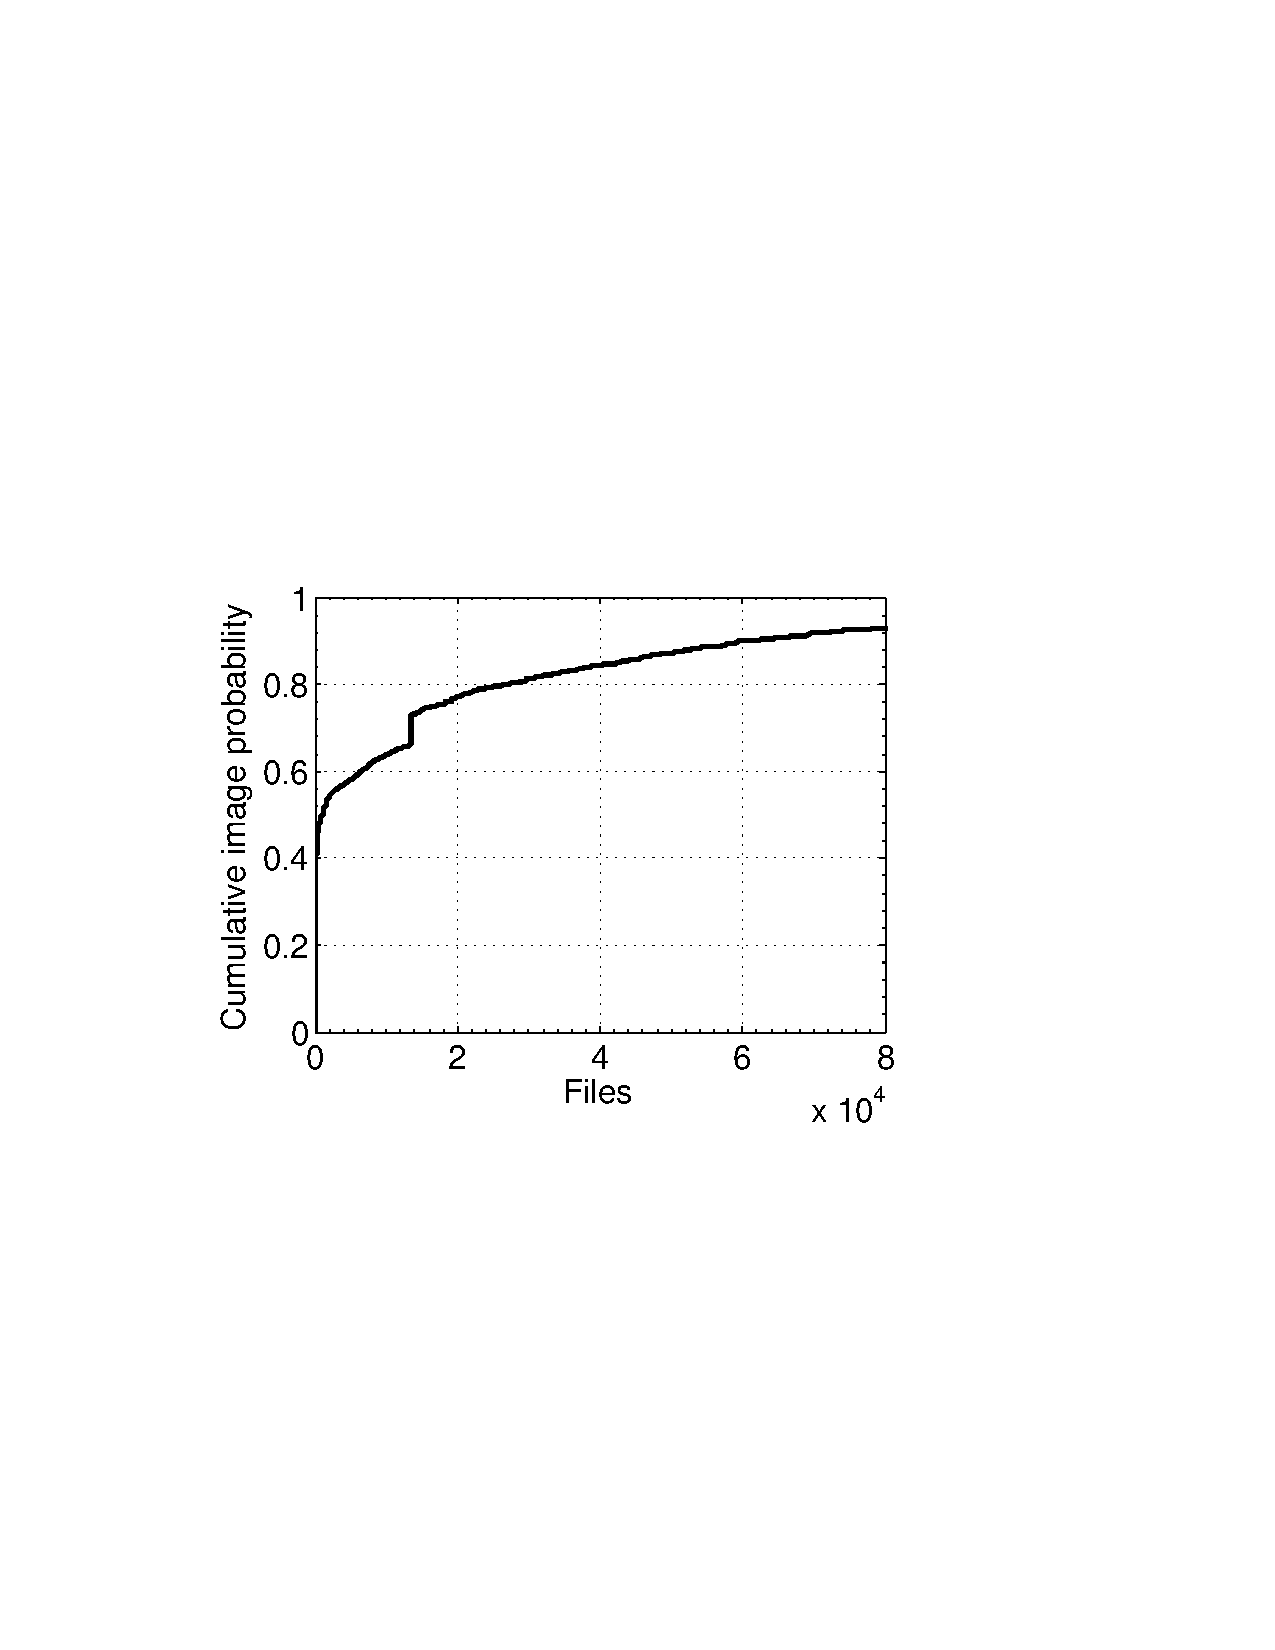
\includegraphics[width=1\textwidth]{graphs/file.pdf}
%		\caption{CDF of images by files}
%		\label{fig-file}
%	\end{minipage}
%\end{figure}

%\begin{figure}[htbp] 
%	\begin{minipage}{0.5\linewidth} 
%		\centering 
%		\includegraphics{circle} 
%		\caption{A Circle} 
%		\label{fig:circle} 
%	\end{minipage}% 
%	\begin{minipage}{0.5\linewidth} 
%		\centering 
%		\includegraphics{rectangle} 
%		\caption{A Rectangle} 
%		\label{fig:rectangle} 
%	\end{minipage} 
%\end{figure}

\paragraphQ{Is there enough time to reconstruct a layer}
\label{sec:layer-preconstruction}
%
%
%As shown in~\cite{xxx}, layer accesses are heavy skewed.  There are hot layers
%that account for majority of layer accesses.  Hence, we can cache hot layers
%to improve performance.
%
%Once layer accesses can be predicted, deduplicated layers can be restored
%before the \texttt{GET} layer request arrives.
%
%As another optimization we explore if it is possible to preconstruct a 
%deduplicated layer before users issues a \texttt{GET} layer to avoid
%the time spend in layer restoration.
%
We analyze the duration between a \texttt{GET} manifest request and the subsequent
\texttt{GET} layer request, denoted inter-arrival time (IAT).
%
As shown in Figure~\ref{fig:intervals}, the majority of intervals are greater than one second.
%
For example, 80\% of intervals from \texttt{lon} are greater than one second,
whereas, 60\% of the intervals from \texttt{syd} are greater than five seconds. 
%
%Hence, there is a relatively long gap
%between a \texttt{GET} manifest request and the subsequent \texttt{GET}
%layer requests.

There are several reasons for this long gap.
%
First, when fetching an image from a registry,
the Docker client fetches a fixed number of layers in parallel (three by
default) starting from the lowest layers.
%
In the case where an image
contains more than three layers, the upper layers have to wait until the
lower layers are downloaded.
%
This varies the \texttt{GET} layer request arrival time for the registry.
%
%<<<<<<< HEAD
Second, network delay between clients and registry
often accounts for a greater portion of the \texttt{GET} layer latency in cloud
environments, especially for the large layers.
%=======
%Second, the network latency between clients and a registry
%often accounts for a large proportion of the \texttt{GET} layer latency,
%especially in Cloud environments.
%>>>>>>> 5cfa95ad1ce38b7942bffcb37086db33854ab296
%

As we show later (\S\ref{sec:Evaluation}) \sysname
can often reconstruct a layer within a single second.
%
In the case of a small duration between a \texttt{GET} manifest request and its subsequent \texttt{GET} layer requests,
layer preconstruction might not be finished in time. However, even in that case layer preconstruction can still be beneficial because
the layer construction starts before the arrival of a \texttt{GET} layer request.
% which can largely reduce the layer construction overhead in the \texttt{GET} layer request latency.

%In summary, it is feasible to start building a layer for the user before
%the \texttt{GET} layer request arrives.


